%\newpage

%//------ Section 01 -------------------------------------------------------------------------------------------------
\chapter{Particle physics}
\label{chap:ParticlePhysics}
%//-----------------------------------------------------------------------//

Particle physics can fairly be defined as the field of Physics dedicated to the study of fundamental particles and their interactions. The idea that matter is composed of elementary bricks is not contemporary, though; the philosophical foundations of this idea date back to the Hellenic epoch in the Ancient Greece (\upperRomannumeral{5}$^{\text{th}}$ century BC)\footnote{The fathers of the Atomism from the Ancient Greece, Leucippus and Democritus, thought that matter was made of both void and elementary, indivisible corpuscules: atoms.} \cite{pullmanAtomHistoryHuman1998}. With the advent of the scientific method, this concept resurface throughout the \upperRomannumeral{19}$^{\text{th}}$ and \upperRomannumeral{20}$^{\text{th}}$ centuries with, among the most notables, John Dalton's atomic theory\footnote{Apart from the name, it does not share much with the philosophical reasoning from the Ancient Greece.} and the discovery of the electron by Joseph J. Thomson \cite{thomsonXLCathodeRays1897}. Although the first known particle, the electron, was discovered in 1897, research on particle physics gained momentum in the 1950s, thanks to the development of the particle accelerators. These devices made possible to observe high-energy collisions of known particles under controlled laboratory conditions and revealed the existence of dozens of particles: discovery of the pion \cite{lattesProcessesInvolvingCharged1947} and kaon in cosmic rays in 1947 \cite{rochesterdr.EvidenceExistenceNew1947}, followed by the ones of the \rmLambda in 1950 \cite{hopperEvidenceConcerningExistence1950}, the anti-proton in 1955 \cite{chamberlainObservationAntiprotons1955}, the electron and muon neutrinos in 1956 \cite{reinesNeutrino1956} and 1962 \cite{danbyObservationHighEnergyNeutrino1962} respectively, the \rmXi in 1964 \cite{barnesObservationHyperonStrangeness1964a}, etc. In total, more than 30 new particles were found by the early 1960s \cite{serwayModernPhysics2004} and it was still increasing. This particle "zoo" confused physicists for a decade. It is not until the 1970s that, thanks to the interplay between theory and experiment, a model successfully provided a unified description of these hundreds of particles: they are, in fact, composite objects, made of smaller and fewer constituents. This model still represents the best description of the sub-atomic universe to this day, hence its well-deserved name: the Standard Model of particle physics. \\

Throughout this chapter, an effort will be made to provide a historical introduction of the modern particle physics, with a particular attention on the many architects that contributed to its construction. The first section, \Sec\ref{sec:StdModel}, presents the Standard Model starting with some mandatory theoretical aspects. This is followed by the description of the different fundamental particles and interactions, that will ultimately lead to the classification of the elementary particles of the Standard Model. The theory of the strong interaction --- the quantum chromodynamics (QCD) --- will profit of a dedicated sub-section, considering its central role in the present manuscript. The different aspects of this force will be discussed, particularly the QCD phase diagram. One of the fascinating phases of QCD matter consists in state of matter in which quarks and gluons are no longer confined within hadrons: the quark-gluon plasma. Such a state --- supposedly corresponding to the primordial state of the Universe a few micro-seconds after the Big Bang ---  is the heart of the \Sec\ref{sec:QGP}. The formation of the QGP in laboratory will be presented, as well as its experimental signatures. One of them, called the strangeness enhancement, stands out of the others, since it has a central role in the studies described in this manuscript. Finally, this chapter will close on a discussion on the different probes of the QGP in view of the \say{recent} results in elementary systems, namely pp and p-Pb collisions. 


\section{The Standard Model of particle physics}
\label{sec:StdModel}

\subsection{Quantum field theories and fundamental symmetries}
\label{subsec:Theory}

Mathematically speaking, the Standard Model is a (relativistic) quantum field theory (QFT), whose dynamics and kinematics are typically described by a Lagrangian\footnote{The choice of a Lagrangian formulation is motivated, at least partially, by the fact that symmetries in the Lagrangian lead directly to conserved quantities/currents \cite{kochAspectsChiralSymmetry1997}.}. In this formalism, particles are expressed in terms of dynamical fields defined at all points of spacetime \cite{peskinIntroductionQuantumField2018}. The construction of the Standard Model relies strongly on group theory and symmetries (or invariances). In essence, the procedure for building a QFT consists in i) specifying a set of symmetries and their associated symmetry group, and ii) writing down the most general Lagrangian that is renormalizable and satisfies the postulated symmetries \cite{braibantParticlesFundamentalInteractions2012}.

There are different classes of symmetries. A transformation that keeps the Lagrangian invariant and applies simultaneously at all points is called a \textit{global} symmetry. Conversely, a similar transformation that would be applied differently at each point is a \textit{local} symmetry. Both global and local symmetries can also be \textit{continuous} if the transformation consists in a sum of infinitemisal transformations -- typically described by Lie groups -- or \textit{discrete} and represented by finite groups \cite{peskinIntroductionQuantumField2018}\footnote{There is also an additionnal difference concerning the quantum numbers: for a continuous symmetry, quantum numbers are additives; for a discrete one, they are multiplicatives \cite{braibantParticlesFundamentalInteractions2012}.}. Continuous symmetries are particularly interesting because of the Noether's theorem \cite{noetherInvariantVariationProblems1971} that fundamentally states: to every continuous symmetry, there corresponds a conserved physical quantity (and vice versa).\\

All QFTs assume global Poincaré invariance, that involves spacetime translations and global Lorentz transformations including rotations in space and boosts. All these symmetries are continuous, and result in the conservation of momentum, energy, angular momentum and the speed of light respectively. The key elements that defines the Standard Model stem, in fact, from a subset of continuous and local symmetries: the \textit{gauge} invariances. Each of these internal symmetries is associated to a certain number of group generators, from which emerge (vector) fields -- called the \textit{gauge} fields --
describing a fundamental interaction. Intuitively, a gauge symmetry corresponds to an invariance under a change of scale or, in other words, of \textit{gauge} \cite{DefinitionGAUGE2023}. For example, the electrostatic field depends on the potential difference and not the potential itself. This means that the electrostatic field is invariant under a shift of the potential. Additionnally, the potential is defined within an additive constant, which corresponds to a \textit{global gauge} \cite{braibantParticlesFundamentalInteractions2012}.

Finally, the Standard Model also relies on discrete symmetries: parity (P), time reversal (T) and charge conjugation (C). Although, most of the interactions preserve these three transformations, this must not be taken for granted. In the current state of the Universe, they are all broken and only the combination of C, P and T still holds as an exact symmetry of Nature \cite{sozziTestsDiscreteSymmetries2019}. That is closely connected with the Lorentz invariance via the so-called CPT theorem \cite{lehnertCPTSymmetryIts2016}, which states that any unitary, local, Lorentz-invariant quantum field theory in a flat Minkowski spacetime must also be CPT invariant and vice-versa \cite{lehnertCPTSymmetryIts2016}\cite{sachsPhysicsTimeReversal1987}. This being said, one can easily imagine that CPT invariance stands as one of the most sacred symmetry in the Standard Model. One of the implication of the CPT theorem involves the properties of matter and antimatter: since the combination C, P and T consists in a mirror-image transformation of particles into antiparticles, the CPT symmetry imposes that they share the same invariant mass, energy spectra, lifetime, coupling constants, etc  \cite{lehnertCPTSymmetryIts2016}\cite{schotterMultidifferentialInvestigationStrangeness2023}.

\subsection{Particles and fundamental interactions}
\label{subsec:ParticleAndInteractions}

The Standard Model provides a description of the fundamental constituents of the observable Universe, the \textit{elementary particles}, and their interactions, the  \textit{forces}. This description encompasses three of the four known fundamental forces: electromagnetic, strong and weak interactions. Gravity is not included for two reasons: on the theoretical side, this force is governed by the laws of general relativity. Its description within an unified framework with the three other interactions turns out to be a difficult -- if not impossible -- task. Furthermore, the coupling strength of gravity is by far the weakest of all the known forces, making it impossible to study experimentally at microscopic scales. \Tab\ref{tab:ForceAndStrength} compiles some properties of the different forces.

The strong interaction, as the name suggests, is the strongest of the four fundamental forces; it is responsible for the cohesion of protons, and neutrons inside the nuclei (also called the nuclear force), for more than 99\% of the observable mass in the Universe and for the confinement of the quarks (explained later in this section and in \ref{subsubsec:confinement}). It has a limited range, though, of only a few \fm. On the opposite side, the weakest of the non gravitational forces is the weak interaction, which also has the shortest effective range (about less than a \fm). The radioactive decay --  as well as the decay of the particles studied in this thesis -- and the fusion of atoms in the Sun originate from this force. Finally, the electromagnetic interaction is certainly the one we are the most familiar with; its coupling strength is in between the strong and weak forces, its range is infinite.\\

\begin{table}[!h]
    \centering
    \begin{tabular}{b{3cm}@{\hspace{1cm}} b{2cm}@{\hspace{0.75cm}} b{2cm}@{\hspace{0.75cm}} b{2.5cm}@{\hspace{0.75cm}} b{1.4cm}@{\hspace{0.75cm}}}
    \noalign{\smallskip}\hline\noalign{\smallskip}
    \bf Interaction (Force) & \bf Particles Acted on by Force & \bf Relative Strength & \bf Typical Lifetimes for Decays via a Given Interaction & \bf Range of Force \\
    \noalign{\smallskip}\hline \noalign{\smallskip}    
    Strong & Quarks, & 1 & $\leq 10^{-20}$ \second & 1 \fm \\
	 & hadrons &  & & \\
    Electromagnetic & Charged & $\approx 10^{-2}$ & $\approx 10^{-16}$ \second & $\infty$ \\
    	 & particles &  & & \\
    Weak & Quarks,  & $\approx 10^{-6}$ & $\geq 10^{-10}$ \second & $10^{-3}$ \fm \\
    	 & leptons &  & & \\
    Gravitational & All & $\approx 10^{-43}$ & ? &  $\infty$ \\
        	 & particles &  & & \\
    
    \noalign{\smallskip}\hline\noalign{\smallskip}
    \end{tabular}
    \caption{The four fundamental interactions, with their corresponding relative strengths, typical lifetime for a decay and range. The relative strenghts are indicative values; obviously, they depend on the distance and energy scale considered. Here, they have been calculated for two particles at a distance of 0.03 \fm. Table taken from \cite{serwayModernPhysics2004}.}\label{tab:ForceAndStrength}
\end{table}

These forces act on the fundamental constituents of matter, the quarks\footnote{The term is apparently inspired from Joyce's book \textit{Finnegans Wake}:"Three quarks for muster Mark..." \cite{s.glashowInteractionsJourneyMind1990}.} and leptons\footnote{From the Greek \textit{leptos} meaning "small" to designate particles of small mass. Nowadays, any fermion that is insensitive to the strong interaction is tagged as a lepton \cite{s.glashowInteractionsJourneyMind1990}.}, which are point-like fermions of spin 1/2. They are twelve organised in three families or generations, each containing two quarks with fractional electric charges (one with $+2 e /3$ and the other with $-1 e/3$, where $e$ corresponds to the electric charge of the positron), one charged lepton and a neutrino\footnote{From the Italian "neutro" for "neutral" and the suffix "ino" for "tiny one",  so "neutrino" means the "tiny neutral one" \cite{s.glashowInteractionsJourneyMind1990}.}. The first family (or generation \upperRomannumeral{1}) consists of the up and down quarks, the electron and the electron neutrino. These are the elements that characterize our low-energy Universe: the quarks make up the nucleons, forming the atomic nuclei, and with the electrons, they constitute the basic building blocks of all earthly matter. The electron-neutrino also plays a role in our everyday Universe, although an indirect one. Without its existence, the primordial hydrogen could not have been transformed into a variety of light and vital elements \cite{kimElectronNeutrinoDegeneracyPrimordial1997} for the development of life. The particles belonging to the first family can be duplicated to form the second and third families. Higher-generation particles have the exact same physical properties as their first-generation cousins, except for the mass that increases with the generation. Because of this difference, fermions from second and third generations tend to go through a chain of decay processes in order to reach particles from the first family. This is why ordinary matter is generally constituted of first-generation particles. I say \textit{generally} because there are two subtleties when it comes to neutrinos: i) since they only interact via weak interaction and gravity, they cannot aggregate to form ordinary matter\footnote{Because the weak interaction only acts at a short distance, and the intensity of the gravitational force is minuscule considering the extremely small mass of neutrinos.} and ii) they can oscillate from one flavour to another, giving rise to the phenomenon of neutrino oscillation. 

A final aspect concerns the \textit{chirality} of the fermions, that is traditionnally introduced by concept of the helicity or handedness. Both are equivalent in the ultra-relativistic limit. On one hand, a particle exists in two versions: \textit{right-handed} if the direction of spin coincides with the direction of motion; \textit{left-handed} if the directions of spin and motion are opposite \cite{thomsonModernParticlePhysics2013}. On the other hand, the chirality also has its own \textit{left-} and \textit{right-handed} states but the concept is more abstract. The chirality determines under which representation of the Poincaré group the particle transforms \cite{QuantumDiaries}.\\

\begin{figure}[h]
	\centering
	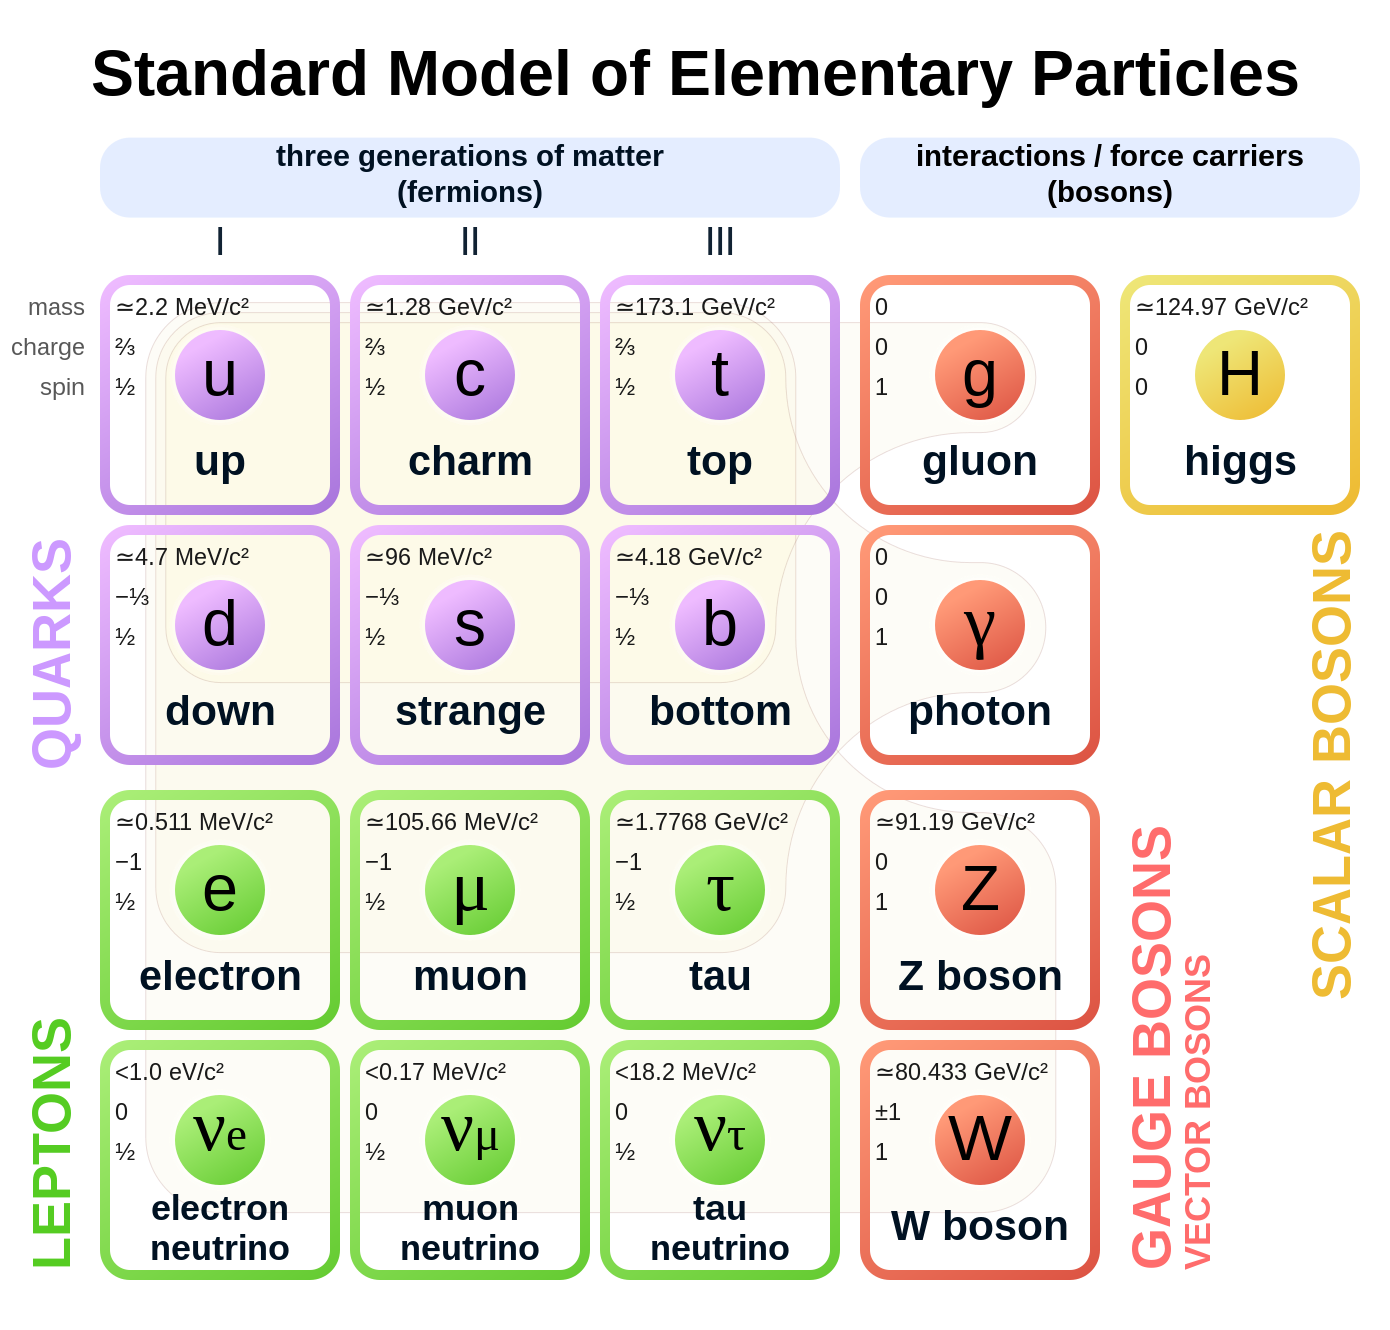
\includegraphics[width=\textwidth]{Figs/Chapter2/Standard_Model_of_Elementary_Particles.svg.png}\label{fig:StdModel}
	\caption{Classification of the elementary particles of the Standard Model, with the fermions on the left and the gauge/scalar bosons on the right. Figure taken from \cite{missmjStandardModelElementary2019}.}
	\label{fig:StdModel}
\end{figure}

Classically, a particle interacts with another via a field (for example, in electromagnetism, a positively charged particle generates an electric field that exerts an attractive/repulsive force on neighboring negative/positive charge). In QFT, fields are quantized, and the energy and momentum previously carried by the field are now conveyed by chunks, by quanta\footnote{Here, we present elementary particles as quanta  of their underlying field as if the particles could be separated/reduced from their field, which corresponds to the usual experimentalist's picture of QFT. In fact, the relation between particles and fields is slightly more subtle \cite{jaegerElementaryParticlesQuantum2021}.} \cite{serwayModernPhysics2004}. So in particle physics, interactions are described as an exchange of quanta or force-carrying particles of spin 1, known as \textit{(vector) gauge bosons}\footnote{They are called \textit{bosons} because, contrarly to the fermions, their intrinsic angular momentum (or spin) has an integer value.}\cite{braibantParticlesFundamentalInteractions2012}\cite{thomsonModernParticlePhysics2013}. Following the remarks in \Sec\ref{subsec:Theory}, the term "(\textit{vector}) \textit{gauge}" emphasizes here the fact that the boson arises from a gauge vector field and therefore a gauge symmetry. 

The most precise quantum field theory is the quantum electrodynamics (QED) that describes the interaction between charged particles and electromagnetic fields. It has been developped between 1947 and 1949 by Shin'-ichir$\bar{\text{o}}$ Tomonaga, Julian Schwinger, Richard P. Feynman and Freeman Dyson; only the first three received the 1965 Nobel Prize in Physics for their contributions\footnote{Unfortunately F. Dyson did not receive the Nobel Prize because i) his work was not considered as groundbreaking as the one of the three other laureates and ii) the Nobel Prize in a given field can only be awarded to organisation of maximum of three individuals \cite{schmidhuberEvolutionNationalNobel2010}.}. It is based on a U(1) local gauge symmetry\footnote{U(N) corresponds to the group of all unitary matrices to size $N \times N$. Thus, U(1) is a group containing all the continuous transformations of the phase of a complex number.}, that results into an interaction with charged particles mediated by massless photons. This continuous symmetry is associated to a conserved quantity, namely the electric charge. The dynamics of this interaction is given by the Lagrangian density of QED in \eq\ref{eq:LagrangianQED}.

\begin{equation}
\Lagr_{QED} = \underbrace{i \bar{\psi} \gamma^{\mu} \partial_{\mu} \psi}_{\substack{\text{electron} \\ \text{kinetic term}}} + \underbrace{e \bar{\psi} \gamma^{\mu} A_{\mu} \psi}_{\substack{\text{electron-photon} \\ \text{interaction term}}} - \underbrace{m \bar{\psi} \psi}_{\substack{\text{electron} \\ \text{ mass term}}} - \underbrace{\frac{1}{4} F_{\mu \nu} F^{\mu \nu}}_{\substack{\text{photon} \\ \text{kinetic term}}} 
\label{eq:LagrangianQED}
\end{equation}
where
\begin{itemize}
\item[$\bullet$] $\gamma^{\mu}$ Dirac matrices that express the vectorial nature of the interaction and $\mu$ is the Lorentz vector index,
\item[$\bullet$] $A_{\mu}$ the photon field,
\item[$\bullet$] $F_{\mu \nu} = \partial_{\mu} A_{\nu} - \partial_{\nu} A_{\mu}$ the field-strength tensor,
\item[$\bullet$] $e$ the coupling constant of QED which coincides with the electric charge of the electron-positron field,
\item[$\bullet$] $m$ the electron/positron mass,
\item[$\bullet$] $\psi$ the electron-positron spinor field,
\end{itemize}
with the Einstein's notation $x^{\mu} x_{\mu} = \sum\limits_{\mu=0}^{N} x^{\mu} x_{\mu}$ and the notations from \cite{thomsonModernParticlePhysics2013}.\\

Different terms appear in the expression of the Lagrangian density: the density of kinetic energy of the spinor field, the density of potential energy due to the interaction between the spinor and gauge fields, the mass energy of the spinor field\footnote{If the gauge boson is massive, there would be an extra mass term. Since the photon is massless, this term is null.}, the density of kinetic energy of the gauge boson (photon). The most interesting term is the second one, which describes the interaction between the charged particles and the photons. This interaction gives rise to different processes, usually pictured by Feynman diagrams. \Fig\ref{fig:FeynmanDiagramQED} shows the basic interaction vertex in QED.

\begin{figure}[H]
\begin{center}
\unitlength = 1mm
\subfigure[]{
	\begin{fmffile}{eegamma}
	\begin{fmfgraph*}(40,25)
	\fmfleft{i1,i2}
	\fmfright{o1}
	\fmflabel{$e^{-}$}{i1}
	\fmflabel{$e^{+}$}{i2}
	\fmf{fermion}{i1,v1}
	\fmf{fermion}{v1,i2}
	\fmf{photon,label=$\gamma$}{v1,o1}
	\end{fmfgraph*}
	\end{fmffile}
	\label{fig:eegamma}
}
\subfigure[]{
	\begin{fmffile}{lqlqgamma}
	\begin{fmfgraph*}(40,25)
	\fmfleft{i1,i2}
	\fmfright{o1}
	\fmflabel{$l, q$}{i1}
	\fmflabel{$\bar{l}, \bar{q}$}{i2}
	\fmf{fermion}{i1,v1}
	\fmf{fermion}{v1,i2}
	\fmf{photon,label=$\gamma$}{v1,o1}
	\end{fmfgraph*}
	\end{fmffile}
	\label{fig:lqlqgamma}
}
\end{center}
\caption{Interaction vertex in QED: (a) involving an electron and a positron, (b) generalized to any charged particles.}
\label{fig:FeynmanDiagramQED}
\end{figure}



Being the first quantum field theory developed, QED paved the way -- and even served as a template -- for all the subsequent quantum field theories. Therefore, it is not surprising that the form of Lagrangian density is the same for all the forces. 

Following the success of QED, attempts to develop a quantum field theory for the weak interaction started in the 1950s; none of them could provide a satisfactory description. In the same decade, important discoveries have been made: the Wu's\footnote{Awarded of the 1957 Nobel Prize.} (1956) and Goldhaber's (1957) experiments \cite{wuExperimentalTestParity1957}\cite{goldhaberHelicityNeutrinos1958} showed that the P- and CP-symmetries are violated by the weak interaction. These led to conclude that this force has a vector-axial vector structure, meaning that only interacts with left-handed chiral particles and right-handed chiral anti-particles. Meanwhile, a few physicists -- including Abdus Salam, Steven Weinberg, Schwinger and his PhD student Sheldon L. Glashow -- foresaw that the weak and electromagnetic forces might be two aspects of the same phenomenon. Thanks to the work of Chen Ning Yang and Robert Mills on the development of a generalized gauge theory in 1954, Glashow delivered the electroweak interaction in 1961, which was consolidated later in 1967 and 1968 by Weinberg and Salam\footnote{For their contribution, Glashow, Salam and Weinberg receive the 1979 Nobel Prize.} respectively. In this quantum field theory, the electromagnetic and weak forces are described within an unified framework; the weak interaction is based on the SU(2) gauge group\footnote{The S (for "special") refers to the group of all matrices whose determinant is equal to 1.}, three generators hence three gauge bosons: \rmWplus, \rmWminus and \rmZzero. These bosons exhibit two unique properties.  First, contrarly to all other gauge bosons, these ones have an enormous mass (m$_{\textrm{W}^{\pm}}$ = 80.377 \gmass and m$_{\textrm{Z}^{0}}$ = 91.1876 \gmass \cite{particledatagroupReviewParticlePhysics2022}), which explains why the weak force is such a short-range interaction. Second, the \rmWplusminus bosons can change the flavour of quarks and leptons. The trend (or the probability) of the flavour-changing is given by the \textbf{C}abibbo-\textbf{K}obayashi-\textbf{M}askawa\footnote{The Universe is unfair: similarly to Dyson for the QED, Nicolas Cabibbo (the pioneer of the CKM matrix) was not awarded with the 2008 Nobel Prize, while Makoto Kobayashi and Toshihide Maskawa were.} (CKM) matrix \cite{particledatagroupReviewParticlePhysics2022}\footnote{Mathematically speaking, this matrix relates the mass eigenstates to the weak eigentstates \cite{thomsonModernParticlePhysics2013}.} in \eq\ref{eq:CKMmatrix}.

\begin{equation}
V_{\textrm{CKM}} = 
\begin{pmatrix}
V_{\rm ud} & V_{\rm us} & V_{\rm ub}\\
V_{\rm cd} & V_{\rm cs} & V_{\rm cb}\\
V_{\rm td} & V_{\rm ts} & V_{\rm tb}
\end{pmatrix} = 
\begin{pmatrix}
0.97425 \pm 0.00022 & 0.2253 \pm 0.0008 & 0.00413 \pm 0.00049\\
0.225 \pm 0.008 & 0.986 \pm 0.016 & 0.0411 \pm 0.0013\\
0.0084 \pm 0.0006 & 0.040 \pm 0.0027 & 1.021 \pm 0.032
\end{pmatrix}\label{eq:CKMmatrix}
\end{equation}

Each matrix element provides the probability of transition from one flavour $i$ to another $j$ for quarks, but the same exists for the leptons and is called the \textbf{P}ontecorvo-\textbf{M}aki-\textbf{N}akagawa-\textbf{S}akata (PMNS) matrix. The elements of the PMNS matrix are slightly different from the CKM ones, though the structure and ordering are the same. 

Finally, concerning the strong interaction, we will see later in its dedicated sub-section, \Sec\ref{subsec:strongforce}. Patience!
\\


The overall picture of the Standard Model's elementary particles is presented in \fig\ref{fig:StdModel}. To this figure should be added the antiparticles. Indeed, to each particle -- fermion or boson -- corresponds an antiparticle that has the same properties, because of the CPT invariance, but with oppositely sign quantum numbers. Consequently, this also means that both CKM and PMNS matrices are the same for particles and antiparticles.

There is, however, one element of the table in the \fig\ref{fig:StdModel} that has not been discussed yet, that is the Higgs boson. It originates from the electroweak unification, so let us retrace our footsteps. The principles of gauge invariance inevitably give rise to massless gauge bosons, like the photons but not the massive \rmWplusminus, \rmZzero bosons. At the time of Glashow's electroweak model in 1961, no one could imagine a mechanism to generate the enormous masses of the weak interaction force-carriers. In the same year, Jeffrey Goldstone showed that the process of spontaneous symmetry breaking\footnote{This is the phenomenon in which a physical system perfectly symmetric breaks the symmetry without any external intervention. The most famous example of such process concerns the magnets. A material can be seen as an ensemble of microscopic magnets. If this material is ferromagnetic, all these magnets will tend to align with their neighbors.  When the temperature increases, the thermal motions start to disrupt this alignement until the material is not magnetized anymore. Conversely, as the material cools down, neighboring magnets starts to align until a critical temperature, when all the magnets lines up in one macroscopic direction. All directions are equivalent but the magnet has to choose one. This choice breaks the symmetic situation when all the directions are equivalent; this is a \textit{symmetry breaking}. Moreover, this choice is not influenced by any external agent, hence it is labelled as \textit{spontaneous}.\label{footnote:SpontaneousSymmetryBreaking}} leads to the existence of massless gauge bosons, called Goldstone bosons. Three years later, in 1964, three independent groups (Robert Brout and François Englert; Peter Higgs; Gerald Guralnik, Carl Richard Hagen, and Tom Kibble) demonstrated the Goldstone bosons could be absorbed by the massless gauge bosons to acquire a mass: this is the Higgs mechanism. It is only in 1967-68, that Weinberg and Salam put to use this mechanism within Glashow's model to generate the masses of \rmWplusminus and \rmZzero bosons. But this goes beyond the scope of the electroweak unification; with this mechanism, the mass of all elementary particles can be generated \cite{s.glashowInteractionsJourneyMind1990}. Incidentally, a new massive spinless particle, associated to a scalar field, emerges out of the Higgs mechanism: the Higgs boson. Its observation in laboratory was at the heart of Standard Model researches for decades until the 14th of March 2013 when the ATLAS and CMS experiments at the LHC at CERN announced the discovery of the Higgs boson \cite{cernNewResultsIndicate2023}\cite{kibbleEnglertBroutHiggsGuralnikHagenKibbleMechanismHistory2009}. The same year, Peter Higgs and François Englert receive the Nobel Prize for their contribution to the Standard Model.


\subsection{The strong force, a colourful interaction}
\label{subsec:strongforce}

Back in the 1960s, in the \say{glorious years} of particle physics, when physicists were submerged by the number of newly discovered \say{elementary} particles. Some of them were subject to the strong interaction, some were not; the former were referred as \textit{hadrons}\footnote{The expression originates from the Greek \textit{adros} meaning "thick and bulky".} and the latter as \textit{leptons}, as discussed in \Sec\ref{subsec:ParticleAndInteractions}. The hadrons were further sorted into two groups known as \textit{mesons} and \textit{baryons}\footnote{These terms originally refer to the mass of the particle: \textit{meson} comes from the Greek root \textit{meso} for "middle", that is in between the electron and proton masses; \textit{baryon} stem from Greek \textit{barys} for "heavy", suggesting any particle with a mass greater or similar to the one of the nucleons. Before the development of the quark model, the difference between the meson and the baryon was driven by their spin. The meson is a boson (integer spin values) where as the baryon is a fermion (half-integer spin values)\cite{s.glashowInteractionsJourneyMind1990}.}. But no one could draw out the underlying scheme between these particles and organise them into some kind of periodic table. There were some attempts though \cite{sakataCompositeModelNew1956}\cite{sakuraiTheoryStrongInteractions1960}; however the Mendeleev of particle physics is arguably Murray Gell-Mann. 

In 1961, he (and independently Yuval Ne'eman) proposed a classification scheme called the \textit{eightfold way} \cite{gell-mannEIGHTFOLDWAYTHEORY1961}\cite{neemanDerivationStrongInteractions1961}. At that time, eight spinless mesons, eight vector mesons of spin 1 and eight spin 1/2 baryons were known. In each of these octets, a pattern emerges when the hadrons are organized into groups/multiplets of roughly the same mass, a hint of the underlying structure of strong interaction. A year later, the eightfold way is updated and completed with a decuplet formed of spin-$\frac{3}{2}$ baryons. However, one of the ten members of the decuplet was not yet discovered but this periodic table of elementary particles can predict its properties: a mass near the 1675 \mmass, strangeness\footnote{A quantum number introduced by Murray Gell-Mann in 1953 order to explain the \textit{strange} behaviour of some particles, such as kaons \cite{gell-mannIsotopicSpinNew1953}. Any particle with a non-zero strangeness value is dubbed \textit{strange particle}.} of -3 and negatively charged, these are the characteristics of the \rmOmegaM. Its existence is confirmed experimentally in 1964 by the Alternating Gradient Synchrotron at the Brookhaven National Laboratory (BNL)\cite{barnesObservationHyperonStrangeness1964a}, validating the eightfold way once and for all.\\

Within the year of this discovery, Murray Gell-Mann (and independently Georges Zweig) unveiled the symmetry behind the eightfold way: there are no elementary hadrons; they are, in fact, all built out of more fundamental particles named \textit{quarks}. A composite object made of bosons can only lead to a boson whereas, formed by fermions, the object is either a fermion or a boson depending on the number of constituents involved. Hence, the quarks must be fermions of spin one-half, mesons are composed of an even number of quarks, baryons of an odd number. The smallest odd number is one, but i) it does not make sense to say that a composite structure is made of one constituent and ii) we will see later in \Sec\ref{subsubsec:confinement} that a system of one quark is physically impossible. Thus, mesons must be made out of two quarks and baryons out of three; these are the simplest imaginable arrangements. 

Originally, quarks exist in two flavours, \textit{up} ($u$) and \textit{down} ($d$), with fractional electric charges of $+2e/3$ and $-1e/3$ respectively. But an extra flavour was needed to explain the existence of strange hadrons: the strange quark, $s$, is born. It has the same properties as the $d$ quark, except that it is much heavier and it has an assigned strangeness number of -1. Any strange hadrons actually contains one to three $s$ quark, depending on their strangeness. Therefore, the predicted particle by the eightfold way, the \rmOmegaM, corresponds actually to the strangest hadron possible, a baryon with three strange quarks. 

With this particle comes the first difficulty of the quark model. Whatever the particle, it must obey the spin-statistics theorem. Quarks being fermions, the theorem states that two \textit{identical} fermions can not occupy the same quantum states simultaneously. However, \rmOmegaM is constituted of three exactly identical $s$-quark \cite{skandsIntroductionQCD2013}. This problem was overcome by Oscar W. Greenberg \cite{greenbergSpinUnitarySpinIndependence1964}, Moo-Young Han and Yoichiro Nambu \cite{hanThreeTripletModelDouble1965} in 1964-65 that introduced a new quantum number, the colour. Each quark comes in three colours or variants labelled as red ($r$), green ($g$) and blue ($b$). In this way, the spin-statistics problem is solved but new questions arises. If quarks carry a colour, hadrons are a mixture of colours. This is assumed to be an equal mixture of all the colours, such that the hadrons are colourless. How come? Why are there no coloured hadrons? 

Along the same line: in 1966, the main accelerator at the Stanford Linear Accelerator Center (SLAC) becomes operational and starts a program of deep inelastic scattering experiments in order to study the inner structure of nucleons. Based on James Bjorken's \cite{bjorkenCurrentAlgebraSmall2018} and Richard Feynman's  \cite{feynmanBehaviorHadronCollisions1988} calculations, the results of SLAC's experiments, in 1969, showed that the nucleons were made of point-like constituents of spin-$\frac{1}{2}$, dubbed \textit{partons}, behaving as free particles \cite{peskinIntroductionQuantumField2018}. The partons were nothing else than the quarks, and these observations established the validity the quark picture to the whole particle physics community. However, it is curious that the partons seem to behave as free particles but they can not escape the hadron.\\

These questions remain unanswered until 1973. This year had seen the development of Quantum Chromodynamics (QCD) -- the quantum field theory of the strong force -- and the discovery of two of its most salient properties, namely the colour confinement and the asymptotic freedom (discussed in \Sec\ref{subsubsec:confinement}). Fruit of the work of Harald Fritzsch, Heinrich Leutwyler and Murray Gell-Mann \cite{fritzschAdvantagesColorOctet1973}, the QCD describes the interaction between colour-charged objects, namely the partons. It is based on the gauge symmetry group SU(3), which has eight generators, giving rise to eight massless gauge bosons called \textit{gluons}, and imposes the conservation of colour. 

QCD is very similar to QED: the electric charge is replaced by a colour charge, antiparticles carry opposite colour charges, and the eight gluons take the role of the photon. The dynamics of QCD is given by the Lagrangian density in \eq\ref{eq:LagrangianQCD}.\\

\begin{equation}
\Lagr_{QCD} = \underbrace{i \bar{\psi}_{q}^{i} \gamma^{\mu} \delta_{ij} \partial_{\mu} \psi_{q}^{j}}_{\substack{\text{quark} \\ \text{kinetic term}}} + \underbrace{g_{s} \bar{\psi}_{q}^{i} \gamma^{\mu} t_{ij}^{a} A_{\mu}^{a} \psi_{q}^{j}}_{\substack{\text{quark-gluon} \\ \text{interaction term}}} - \underbrace{m_{q} \bar{\psi}_{q}^{i} \psi_{qi}}_{\substack{\text{quark} \\ \text{mass term}}} - \underbrace{\frac{1}{4} F_{\mu \nu}^{a} F^{a \mu \nu}}_{\substack{\text{gluon} \\ \text{kinetic term}}} 
\label{eq:LagrangianQCD}
\end{equation}
where, using the notations from \cite{skandsIntroductionQCD2013},
\begin{itemize}
\item[$\bullet$] $g_s^2 = 4 \pi \alpha_s$ with \alphaS the coupling constant of QCD,
\item[$\bullet$] $F_{\mu \nu}^{a} = \underbrace{\partial_{\mu} A_{\nu}^{a} - \partial_{\nu} A_{\mu}^{a}}_{\text{Abelian part}} + \underbrace{g_{s} f^{abc} A_{\mu}^{b} A_{\nu}^{c}}_{\text{non-Abelian part}}$ the field-strength tensor,
\item[$\bullet$] $\psi_{q}^{i}$ the quark field spinor with colour index $i$ such that $\psi_{q} = \left({\color{red}\psi_{qR}}, {\color{green}\psi_{qG}}, {\color{blue}\psi_{qB}} \right)^{\rm T} $,
\item[$\bullet$] $m_{q}$ the quark \textit{bare} mass induced by the Higgs mechanism,
\item[$\bullet$] $A_{\mu}^{a}$ the gluon field with colour index $a$,
\item[$\bullet$] $t_{ij}^{a} = \frac{1}{2} \lambda_{ij}^{a}$ and $\lambda^{a}$ the fundamental\footnote{The representation of a group is \textit{fundamental} when its generators are hermitian and traceless matrices. } representation of the generator of SU(3) associated to the colour index $a$,
\item[$\bullet$] $f^{abc}$ the structure constants of SU(3).\\
\end{itemize}

As in QED, the Lagrangian density can be expressed with four terms; the quark-gluon interaction is described by the second one. However, the field-strength tensor $F_{\mu \nu}^{a}$ here admits an extra term because the generators of SU(3) do not commute. The non-Abelian property of the gauge group of QCD gives rise to gluon-self interactions, as shown in the Feynman's diagrams of \fig\ref{fig:FeynmanDiagQCD}.

\begin{figure}[H]
\begin{center}
\unitlength = 1mm
\subfigure[]{
	\begin{fmffile}{qqg}
	\begin{fmfgraph*}(40,25)
	\fmfleft{i1,i2}
	\fmfright{o1}
	\fmflabel{$q$}{i1}
	\fmflabel{$\bar{q}$}{i2}
	\fmf{fermion}{i1,v1}
	\fmf{fermion}{v1,i2}
	\fmf{gluon,label=$g$, lab.dist=0.1w}{v1,o1}
	\end{fmfgraph*}
	\end{fmffile}
	\label{fig:qqg}
}
\subfigure[]{
	\begin{fmffile}{ggg}
	\begin{fmfgraph*}(40,25)
	\fmfleft{i1,i2}
	\fmfright{o1}
	\fmflabel{$g$}{i1}
	\fmflabel{$g$}{i2}
	\fmflabel{$g$}{o1}
	\fmf{gluon}{i1,v1}
	\fmf{gluon}{i2,v1}
	\fmf{gluon}{v1,o1}
	\fmfv{lab=$g_s$,lab.dist=0.15w}{v1}
	\fmfdot{v1}
	\end{fmfgraph*}
	\end{fmffile}
	\label{fig:ggg}
}
\subfigure[]{
	\begin{fmffile}{gggg}
	\begin{fmfgraph*}(40,25)
	\fmfleft{i1,i2}
	\fmfright{o1,o2}
	\fmflabel{$g$}{i1}
	\fmflabel{$g$}{i2}
	\fmflabel{$g$}{o1}
	\fmflabel{$g$}{o2}
	\fmf{gluon}{i1,v1}
	\fmf{gluon}{i2,v1}
	\fmf{gluon}{v1,o1}
	\fmf{gluon}{v1,o2}
	\fmfv{lab=$g_s^2$,lab.dist=0.15w}{v1}
	\fmfdot{v1}
	\end{fmfgraph*}
	\end{fmffile}
	\label{fig:gggg}
}
\end{center}
\caption{The three possible interaction vertices within the framework of QCD: (a) quark-gluon, (b) triple-gluon and (c) four-gluon interactions.}
\label{fig:FeynmanDiagQCD}
\end{figure}

Consequently to the self-interaction of QCD's force-carriers, gluons can not be colour neutral. To ensure colour conservation at the interaction vertex in \fig\ref{fig:qqg}, the gluon must carry a colour and an anti-colour charges. This calls for a revision of the term \textit{partons}: it corresponds to any colour-charged elementary particle, that is the quarks \textit{and} gluons. 

Furthermore, quarks are bound together inside hadrons through the exchange of gluons, but because of their self-interaction feature, gluons can radiate other gluons (\fig\ref{fig:ggg}); the latters can, in turn, split into a quark-antiquark pair (\fig\ref{fig:qqg}) or emit gluons again, and so on. The static picture of hadrons  with two or three quarks exchanging gluons turns out to be more complex, permeated in a \textit{sea} of quarks (and antiquarks) and gluons\footnote{An effect of the sea of quarks and gluons is the Bjorken scaling violation observed by the HERA experiment \cite{braibantParticlesFundamentalInteractions2012}\cite{thomsonModernParticlePhysics2013}.}. However, the elements inside the sea do not determine the quantum numbers or properties of the hadron, as opposed to the "original" quarks; for this reason, the latter are often refered as \textit{valence quarks}.

Finally, an incidental consequence of gluon's self-interaction is the running of the coupling constant. This can be understood by making a (anti)parallel with QED. Let us say we want to measure the coupling strength with a charged particle (an electron, for example). In QFT, the vacuum is not entirely empty, it contains pairs of particles and antiparticles that are constantly created and annihilated. Such a pair can also be formed by the cloud of \textit{virtual}\footnote{Certainly the most vague concept in particle physics. It appears in perturbation theory (see later) and an attempt for a definition could be: it corresponds to a theoretical particle wich exhibits the same properties as ordinary particles but not necessarily (for example, they do not satisfy the energy-momentum relation), and with a lifetime so short that it could never be observed experimentally.} photons surrounding the charged particle to be tested; in this case, it is said to \textit{polarise the vacuum}. An example of this process can be found in \fig\ref{fig:ChargeScreening}. The positively charged particle from the vacuum is attracted to the initial electron, leading in a screening effect similar to the one found in a dielectric material (\fig\ref{fig:Dielectric}). At large distance (or small energy), it is more difficult to penetrate inside the cloud of virtual particle-antiparticle pairs and to probe the initial charge, reducing the coupling strength. Conversely, at small distance (or large energy), the initial charge can be distinguished from the surrounding positively charged particles and the coupling strengthen. In QCD, the opposite happens.  Because gluons carry a colour charge, the initial colour of the particle to be tested (a quark) gets spread out, as depicted in \fig\ref{fig:ColourSpread}. Thus, an anti-screening effect occurs: the initial red-coloured quark spends most of its time coloured as blue or green, and the red colour charge is diluted in the surrounding cloud of partons. At large distance (or small energy), the initial quark $r$ is overly apparent for an incoming gluon $\bar{r}g$ or $\bar{r}b$; conversely, at small distance (large energy), the initial red quark -- likely converted into a green or blue quark -- is invisible to such a gluon, resulting in a weakening of the coupling strength. \\

\begin{figure}[t]
\begin{center}
\subfigure[]{
	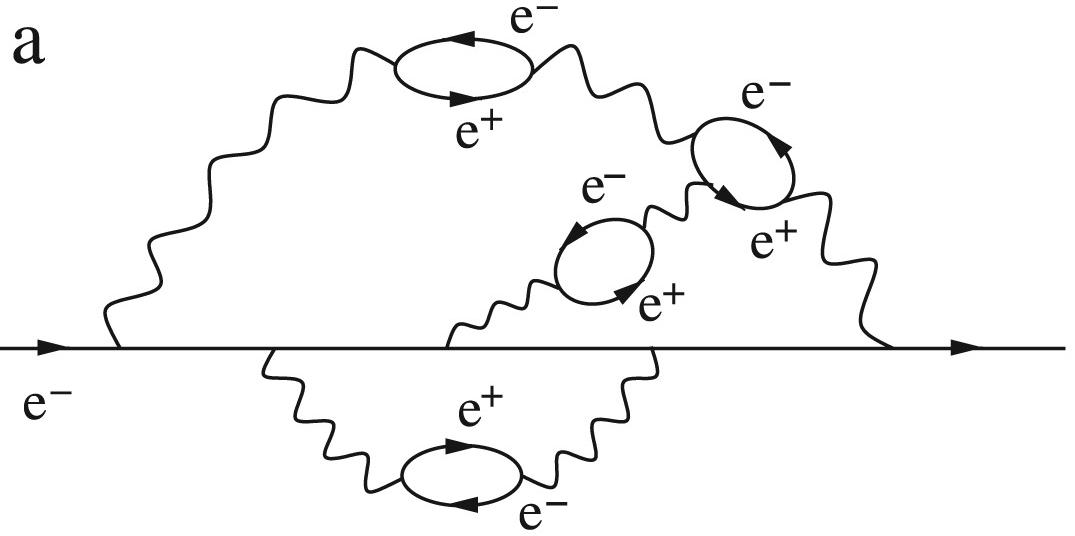
\includegraphics[height=0.25\textwidth]{Figs/Chapter2/1-s2.0-S0146641016300035-gr2_lrg}
	\label{fig:ChargeScreening}
}
\subfigure[]{
	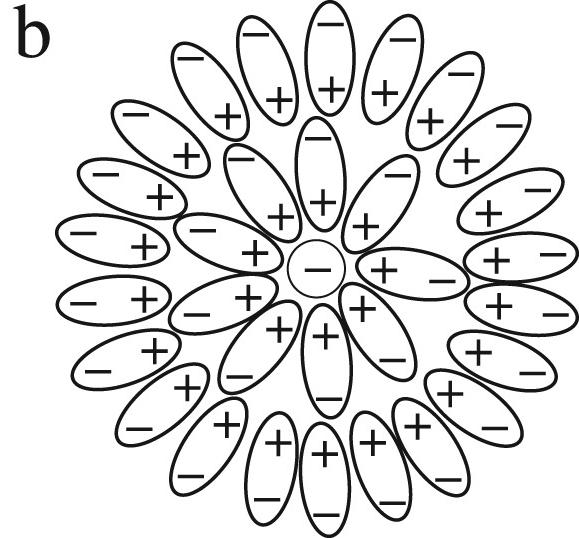
\includegraphics[height=0.25\textwidth]{Figs/Chapter2/1-s2.0-S0146641016300035-gr2bis_lrg}
	\label{fig:Dielectric}
}
\subfigure[]{
	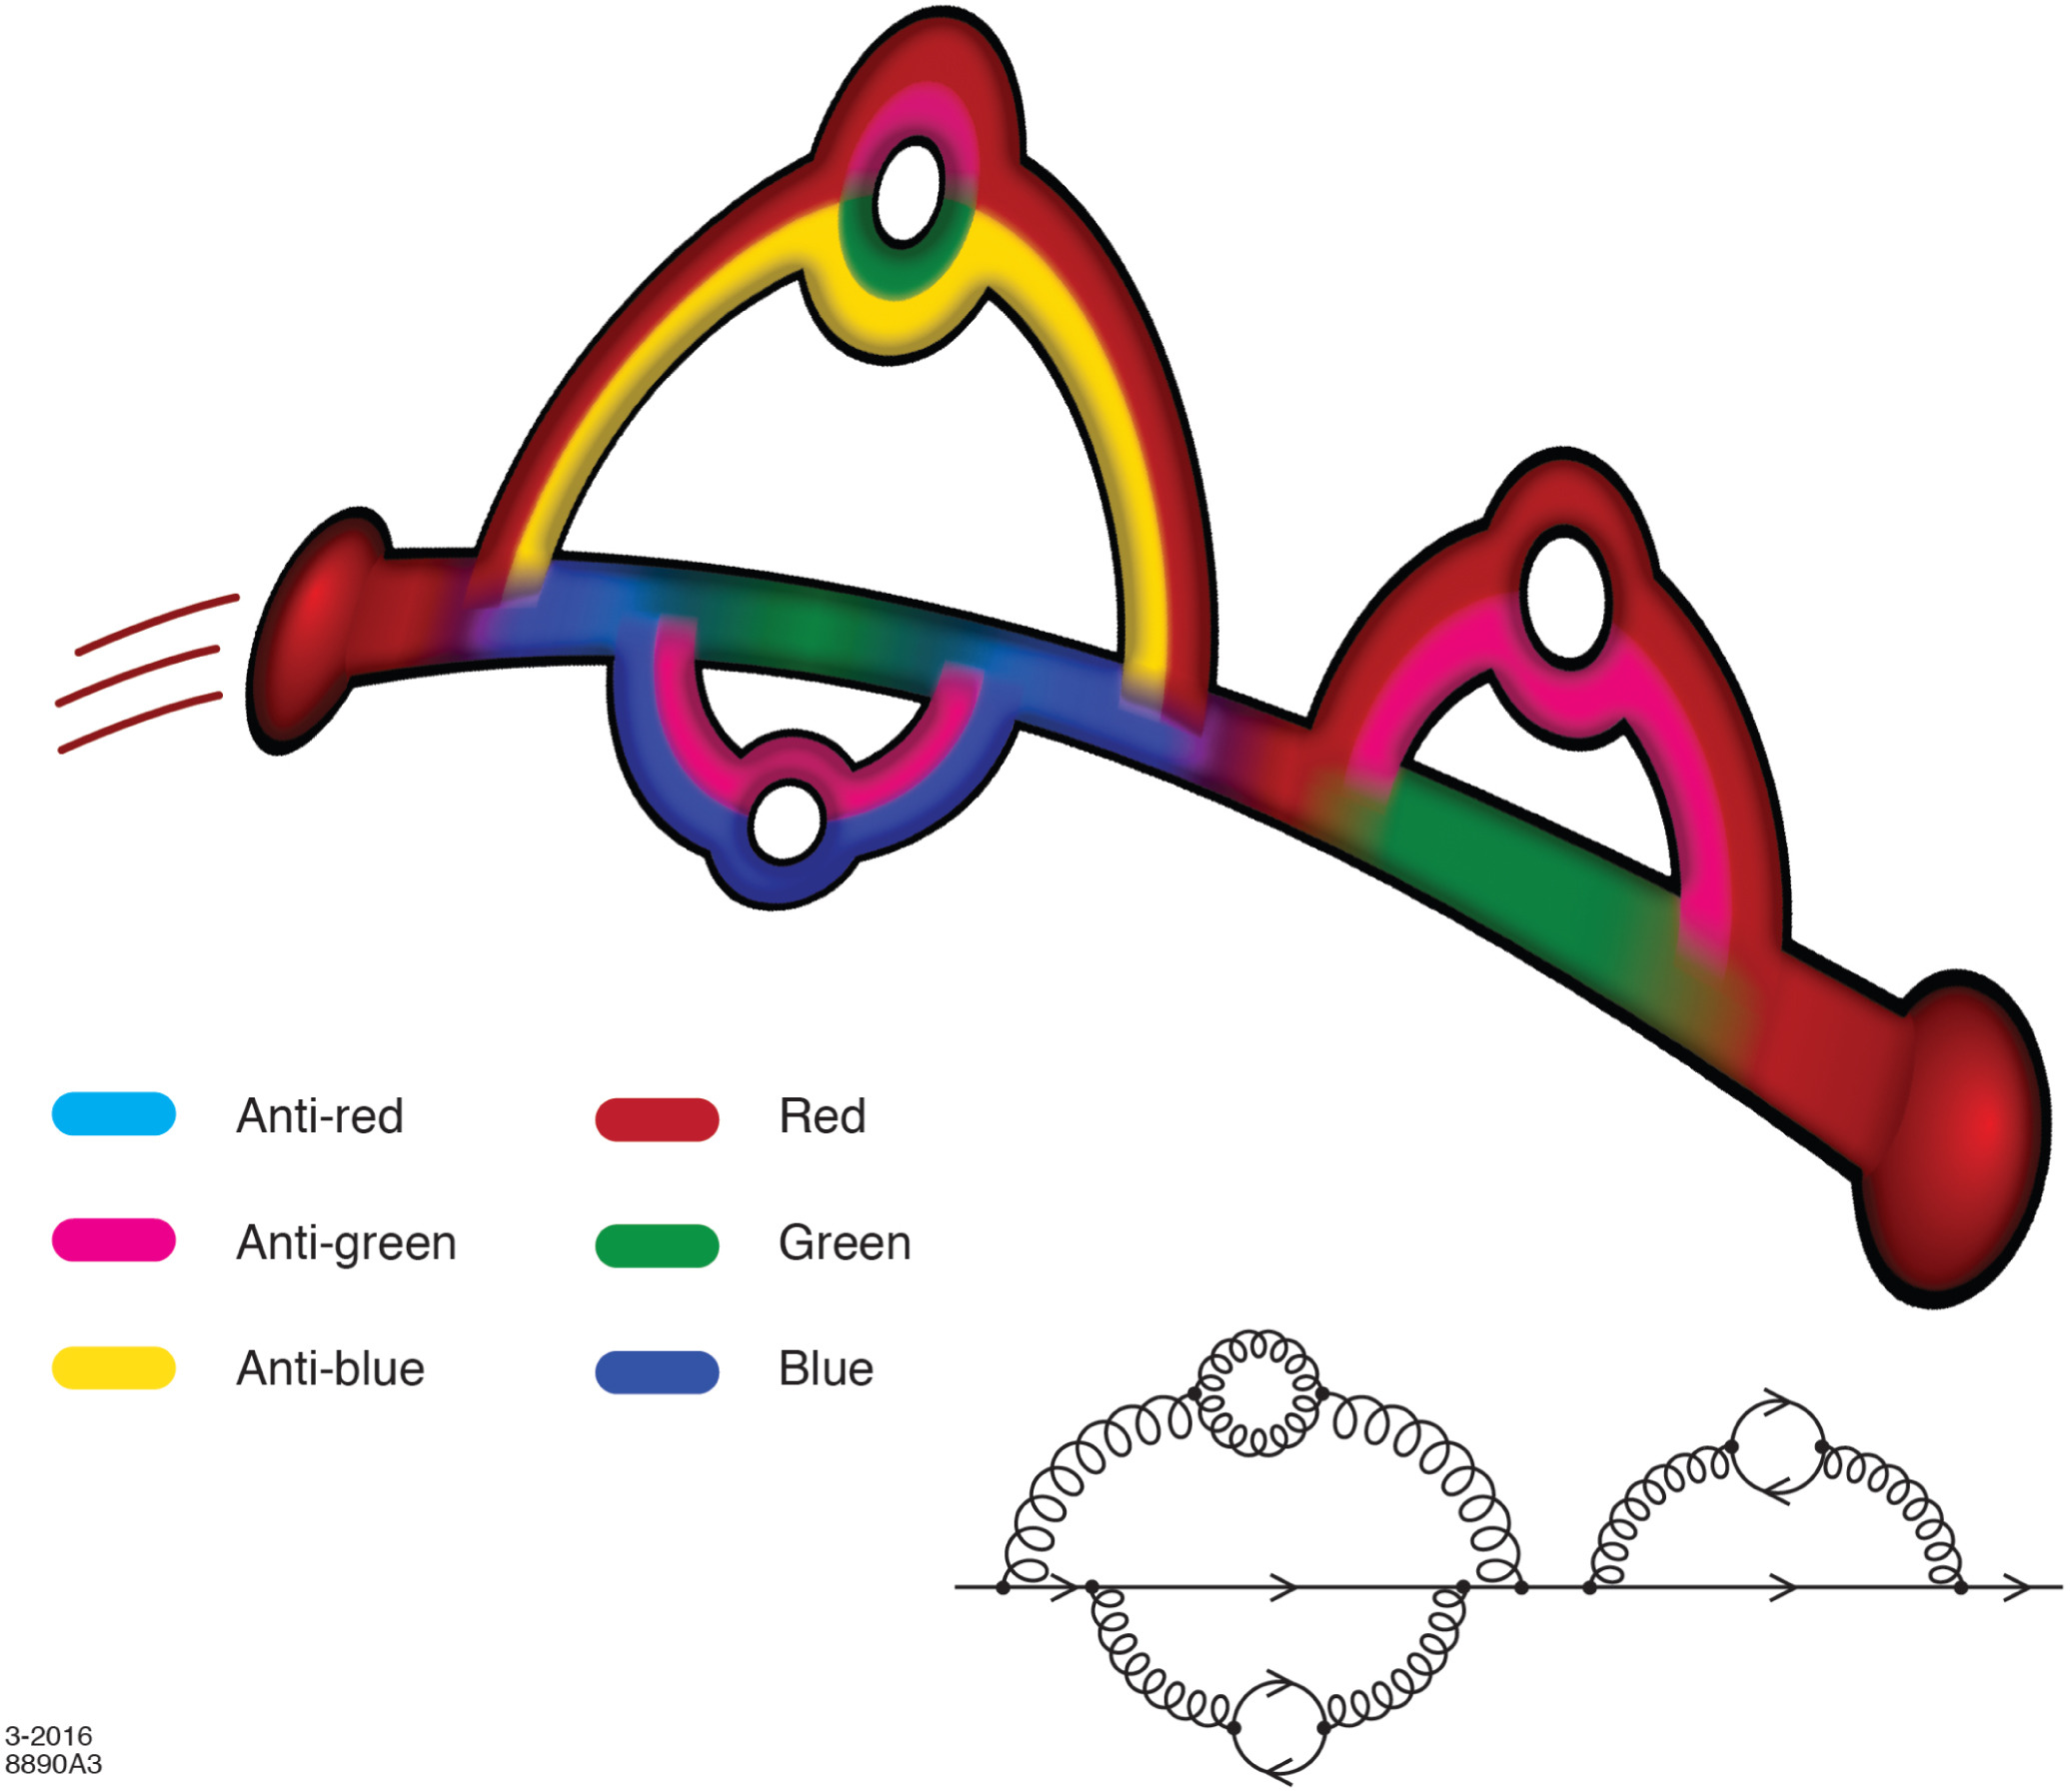
\includegraphics[width=0.8\textwidth]{Figs/Chapter2/1-s2.0-S0146641016300035-gr1_lrg.jpg}
	\label{fig:ColourSpread}
}
\end{center}
\caption{(a) screening effect of an electron in QED, induced ;(b) analogy with the screening effect in a dielectric material; (c) pictural representation of the colour spread of an initially red coloured quark. }
\label{fig:ProbingTestCHarge}
\end{figure}

%A physical picture often used to describe this effect is that a charged particle "polarizes the vacuum", and is "dressed" by a cloud of virtual photons and other charged particles. An electron will attract virtual positively charged particles out of the vacuum that effective screen the electric charge seen by an observer far away from the electron, reducing the size of the coupling. By bringing two charged particles to shorter distances (so they interact at a higher energy), the effective coupling between them is stronger because each charge penetrates the other's cloud, and so the virtual particles swarming in the quantum vacuum are less able to screen the bare charge of each charged particle. The reason for the name "screening" is that (in this picture) the quantum vacuum is screening the bare charge by surrounding it with virtual particles of the opposite charge. I should emphasize that this is a nice physical picture, but ultimately is just a set of words draped around a rigorous calculation of the running of the electromagnetic coupling with energy.

Before continuing, allow me to digress and finish with the different quarks within the QCD framework. The alert reader may have guessed that the story did not end with the strange quark. In 1964, James Bjorken and Sheldon Glashow introduced a new quark flavour: the charm quark. It is motivated by the idea of a quark-lepton symmetry\footnote{The term \textit{charm} is chosen for designating this fourth flavour because the definition found by Bjorken and Glashow in \textit{American Heritage Dictionnary}: "an action or formula thought to have magical power", implying magical power to restore the quark-lepton symmetry \cite{s.glashowInteractionsJourneyMind1990}.} at that time, there was four known leptons (electron, muon and their associated neutrinos) and three quarks. But the charm quark definitely comes into play in 1970 by Sheldon Glashow (again), John Iliopoulos and Lucinao Maiani to explain the strangeness-changing neutral currents\footnote{This is typically the case of the decay of a negative kaon to a negative pion with a neutrino and an anti-neutrino ($\rmKminus \rightarrow \piMinus \nu \bar{\nu}$). It is called a strangeness-changing neutral current because i) the strange particle (kaon) changed into an ordinary one (pion), and ii) there is no electric (or neutral) charge transfer between the hadrons to the leptons. This process was never observed in laboratory, as opposed to the strangeness-changing charged current: ($\rmKminus \rightarrow \piZero e^{-} \bar{\nu}_{e}$). To eliminate the strangeness-changing neutral currents, a new quark flavour needed to be introduced \cite{s.glashowInteractionsJourneyMind1990}.}. Its existence is validated by the observation of the first charmed hadron in 1974 by Burton Richter (SLAC)\cite{augustinDiscoveryNarrowResonance1974} and Samuel Chao Chung Ting (BNL)\cite{aubertExperimentalObservationHeavy1974}; both receive the 1976 Nobel Prize for that discovery. In parallel, a third generation of quark is introduced, in 1972 by Makoto Kobayashi and Toshihide Maskawa\footnote{For the discovery of, at least, a third family of quarks, they both receive the 2008 Nobel Prize.} to explain the observed CP violation. The particles composing this new family make their appearence in 1975, thanks to Haim Harari \cite{harariNewQuarkModel1975}, under the name of \textit{bottom} and \textit{top} quarks\footnote{Both belong to the same weak isospin doublet, as are the down and up quarks. To match the labelling of the first generation of quarks, the names \textit{bottom} and \textit{top} were chosen.}. Evidence of the bottom quark is found in 1977 by Leon M. Lederman at Fermilab \cite{herbObservationDimuonResonance1977}. Due to its large mass, the discovery of the top quark takes more time but ultimately occurs in 1995 by two groups at Fermilab \cite{cdfcollaborationObservationTopQuark1995}\cite{d0collaborationObservationTopQuark1995}.

\subsubsection{Running of \alphaS, colour confinement and asymptotic freedom}
\label{subsubsec:confinement}

\begin{figure}[h]
	\centering
	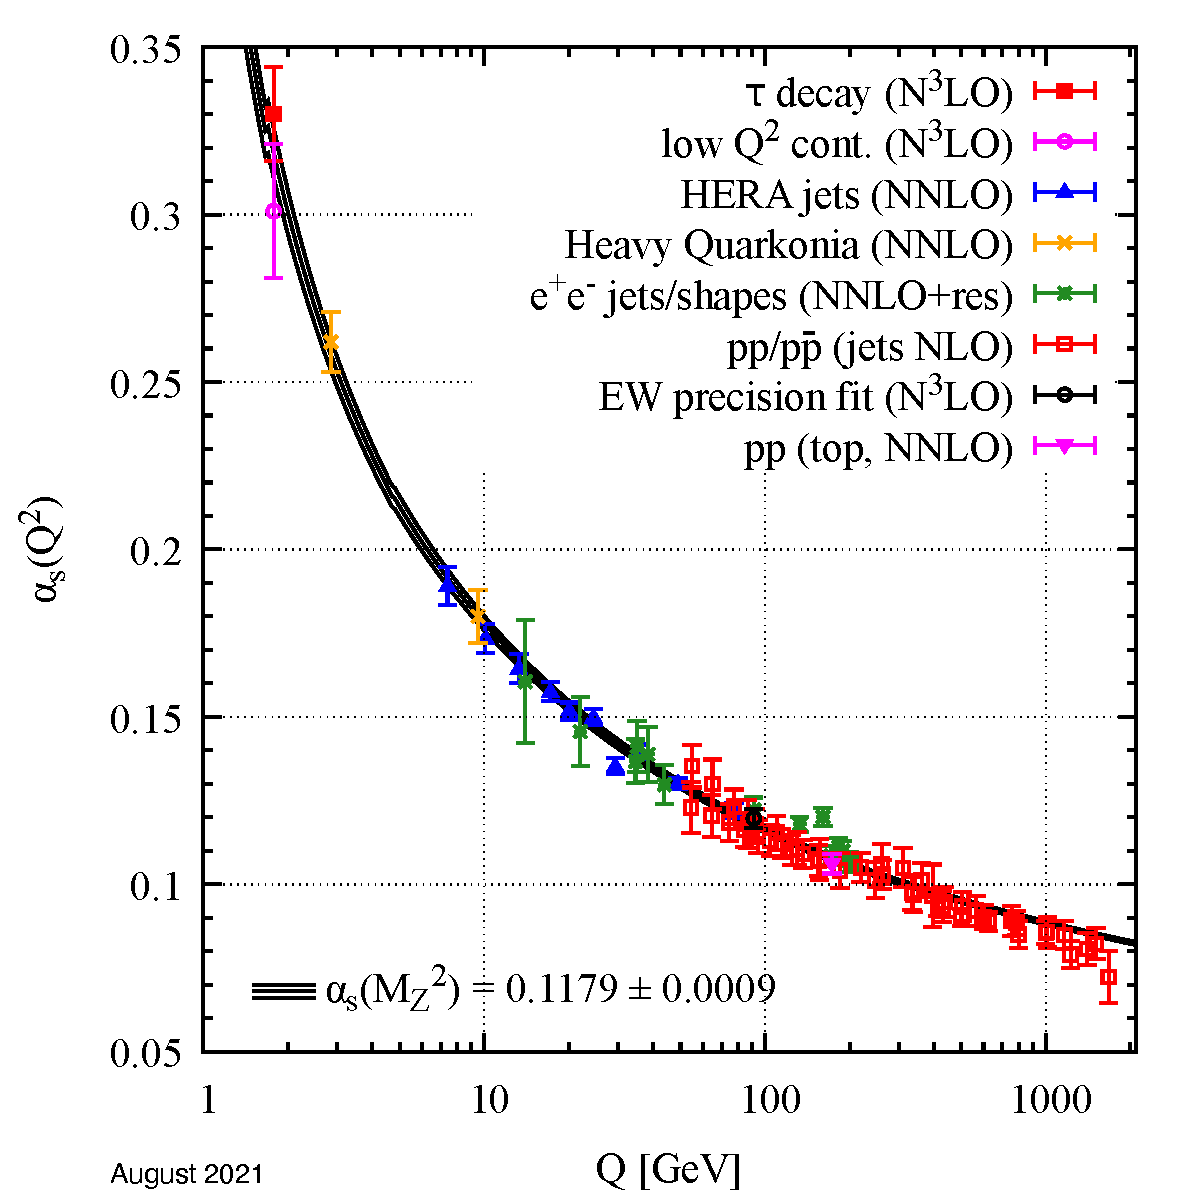
\includegraphics[width=0.8\textwidth]{Figs/Chapter2/alphas-v-Q-2021.pdf}
	\caption{Running of the coupling constant of the strong interaction, \alphaS, as a function of the energy transfer $Q$. The markers represent measurements based on perturbative calculation (the order of the perturbation development is indicated in parenthesis), the solid line corresponds to analytical prediction. Figure taken from \cite{particledatagroupReviewParticlePhysics2022}.}
	\label{fig:RunningAlphaS}
\end{figure}

\Fig\ref{fig:RunningAlphaS} shows the running of the coupling constant \alphaS of QCD as a function of the energy transfer $Q$. The strength of the interaction varies considerably, such that two regimes can be discerned: one at large $Q$ (or small distance) when the strong interaction is "weak" (\alphaS small), the other at small $Q$ (or large distance) when the coupling constant gets "strong" (\alphaS large). Usually, these two regimes are delimited by defining an energy scale, denoted as \LambdaQCD, at which $\alphaS \sim 1$. This corresponds to $\LambdaQCD \sim 200$ MeV\footnote{The definition of \LambdaQCD is convenient because it allows to classify quarks as a function of their mass hierarchy with respect to \LambdaQCD: $u$, $d$ and $s$ quarks belongs to the light-flavour sector ($\LambdaQCD \ll m_{s}, m_{u}, m_{d}$), the others are heavy-flavour quarks ($m_{t}, m_{b}, m_{c} \gg \LambdaQCD$).}. Far above this value, the contribution of high-order diagrams decreases with their order such that most of them can be neglected, and QCD predictions can be calculated easily -- or in the some cases, it simply renders the calculations possible -- using perturbation theory. In this case, we talk about perturbative QCD (pQCD).

As the energy transfer decreases, the coupling constant increases and perturbative calculations starts to diverge until the point where it becomes infinite, at \LambdaQCD. At this value or below, QCD is dominated by the contributions from high-order diagrams and can not be treated perturbatively anymore. The only way out is to perform analytical calculations, which is not possible due to the complexity of QCD. A more viable option is to resort to numerical calculations. A well-established technique is called \textit{lattice QCD}, where to each (space-time) point of the lattice/grid corresponds a spinor field representing the quarks possibly connected (or not) by links describing the gluon vector field. Although it provides some insights on non-perturbative physics aspects of QCD, it is extremely demanding in terms of computational power and time -- these two factors being strongly dependent on the lattice size.\\

A phenomenological approach of QCD, supported by lattice calculations, can also be followed by considering that the interaction potential between two quarks separated by a distance $r$ is approximated by\footnote{The expression of the potential is experimentally motivated by the ordering in the spectra of the charmonium ($c\bar{c}$) and bottomium ($b\bar{b}$) bound states \cite{thomsonModernParticlePhysics2013} \cite{martinParticlePhysics2017}.}
\begin{equation}
V(r) \approx - \frac{\alpha_{s}(r)}{r} + \kappa r,
\label{eq:QCDPotential}
\end{equation}
where the constant $\kappa$ is typically about 1 GeV/fm \cite{martinParticlePhysics2017}. The alert reader recognises the first term as the Coulombian-potential, similar to the one in QED; the second term corresponds to an elastic spring-type force. As illustrated in \fig\ref{fig:QCDPotential}, they describe two specific behaviours of the QCD interaction potential.

\begin{figure}[t]
	\centering
	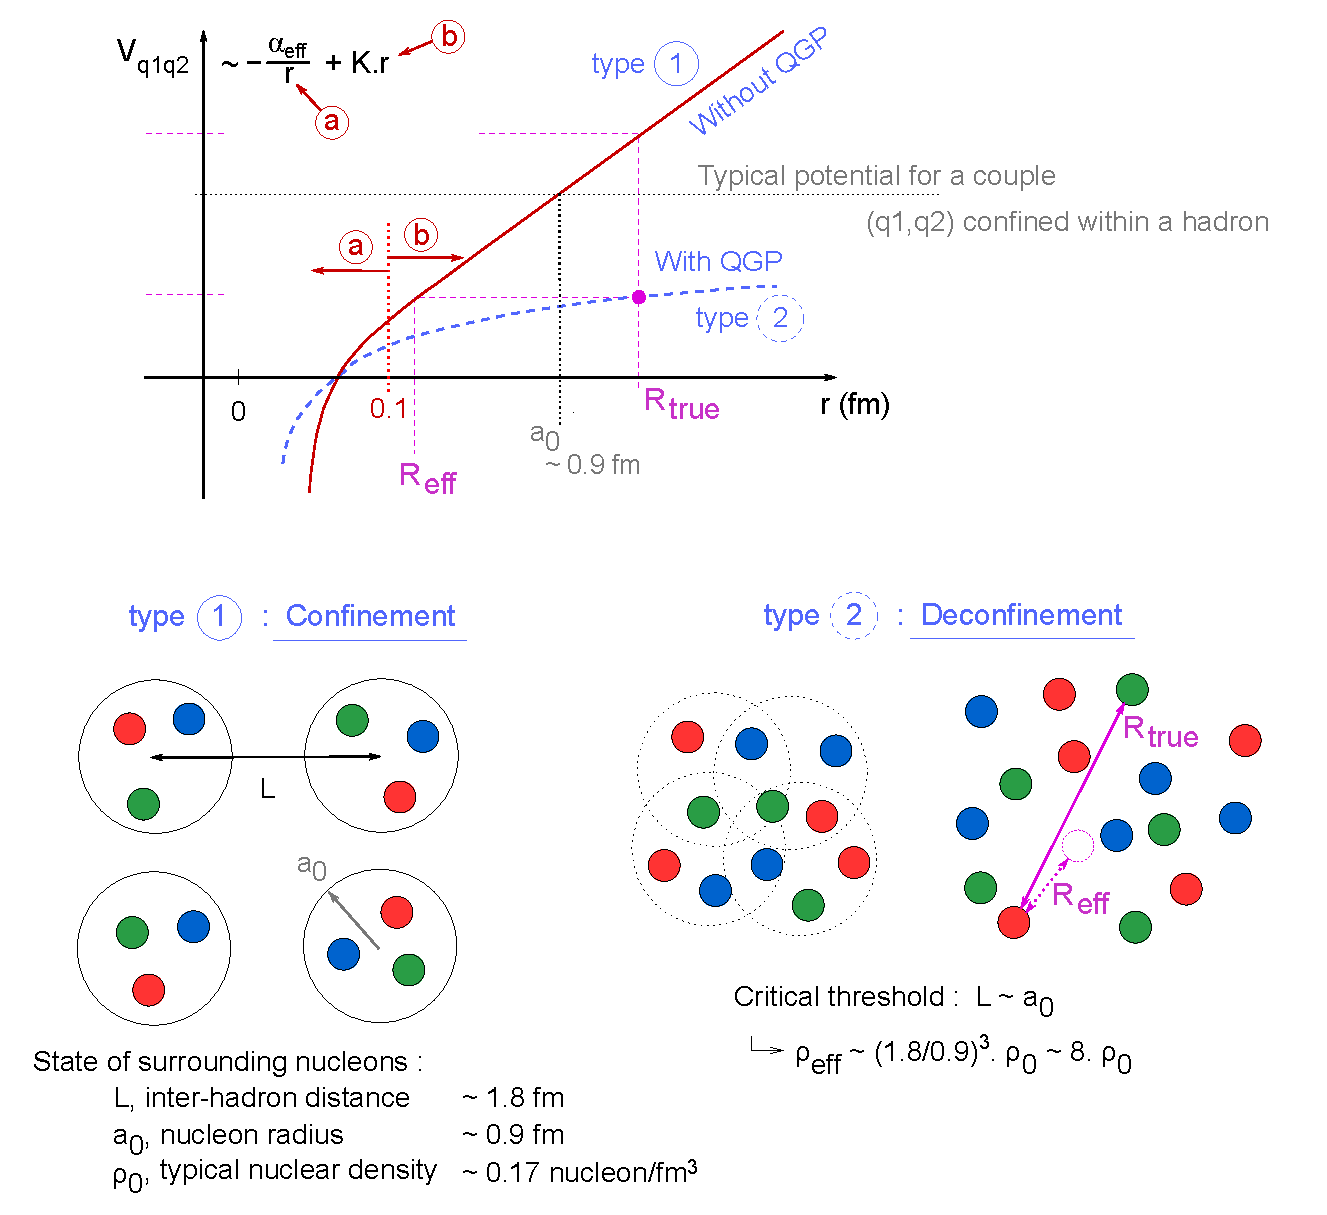
\includegraphics[width=0.9\textwidth]{Figs/Chapter2/GraphePotentiel.eps}
	\caption{QCD interaction potential between two coloured-objects (quark-quark or quark-antiquark) as a function of their separation $r$. Figure taken from \cite{maireProductionBaryonsMultietranges2011}.}
	\label{fig:QCDPotential}
\end{figure}

At small distance ($r \leq 0.1 \fm$), the Coulomb-type term dominates, the interaction potential diminishes asymptotically as the distance decreases; it is not divergent though, as \alphaS also varies. The quarks interacts less and less, and becomes quasi-free. This phenomenon, known as \textit{asymptotic freedom}, has been discovered by David Gross, Frank Wilczek in 1973 \cite{grossUltravioletBehaviorNonAbelian1973} and Hugh David Politzer in 1974 \cite{davidpolitzerAsymptoticFreedomApproach1974}, and sets the groundwork for the development of a quantum field theory of strong interaction, that is the QCD\footnote{In the early seventies, the common belief among the theoreticians was that quantum field theory fails to describe the strong interaction, and therefore it would be impossible to have a common mathematical framework for all the known forces (except gravity) \cite{s.glashowInteractionsJourneyMind1990}.}. Neither the electrostatic force between two charges nor the gravitational force between two masses exhibit this property; in these cases, the interaction gets weaker as the distance increases between the two objects.

Conversely, the second term takes the upper hand at $r \geq 1 \fm$, the force increases linearly with the distance between the two quarks, as if they were connected by an elastic or spring made of gluons. As the quarks are pulled away, the energy stored in the spring of gluons accumulates until it reaches the threshold to create a quark-antiquark pair\footnote{There is an alternative scenario: the energy stored in the spring of gluons continues to increase until it reaches the threshold to create not one but two quark-antiquark pairs. Obviously, this path -- which explains the production of one or several baryons from the vaccum -- demands more energy and thus is less probable to occur.}. This description is shown on \fig\ref{fig:QuarkFragmentation}. The spring tying together the initial $q_{i}\bar{q}_{i}$ pair ruptures and the accumulated energy is expended on producing a $q_{1}\bar{q}_{1}$ pair: the freshly created quark, $q_{1}$, binds with $\bar{q}_{i}$,  $\bar{q}_{1}$ with $q_{i}$. This process continues until all the $q\bar{q}$ pairs have a sufficiently low energy to combine into a hadron. Note that the initial quark-antiquark pair could be replaced by a pair of gluons and the process would still be the same. As a result, any colour-charged particle -- quark or gluon -- can not be found isolated; they must be confined in a colour-neutral object, such as meson and baryon\footnote{If there is (ordinarily...) no such thing as free parton, the same would be true for a colour-charged hadron. For this reason, baryons and mesons are colour-neutral structures.}. This phenomenon is refered as \textit{colour confinement}.


Interestingly enough, the quark confinement is analogous to the behaviour of a magnet. The latter consists of a north and south poles. If one tries to isolate one of the poles, for example, by cutting the magnet in half, this would only yield into two small magnets. Like the quarks, no one has ever seen an isolated magnetic pole (magnetic monopole).

\begin{figure}[t]
\begin{center}
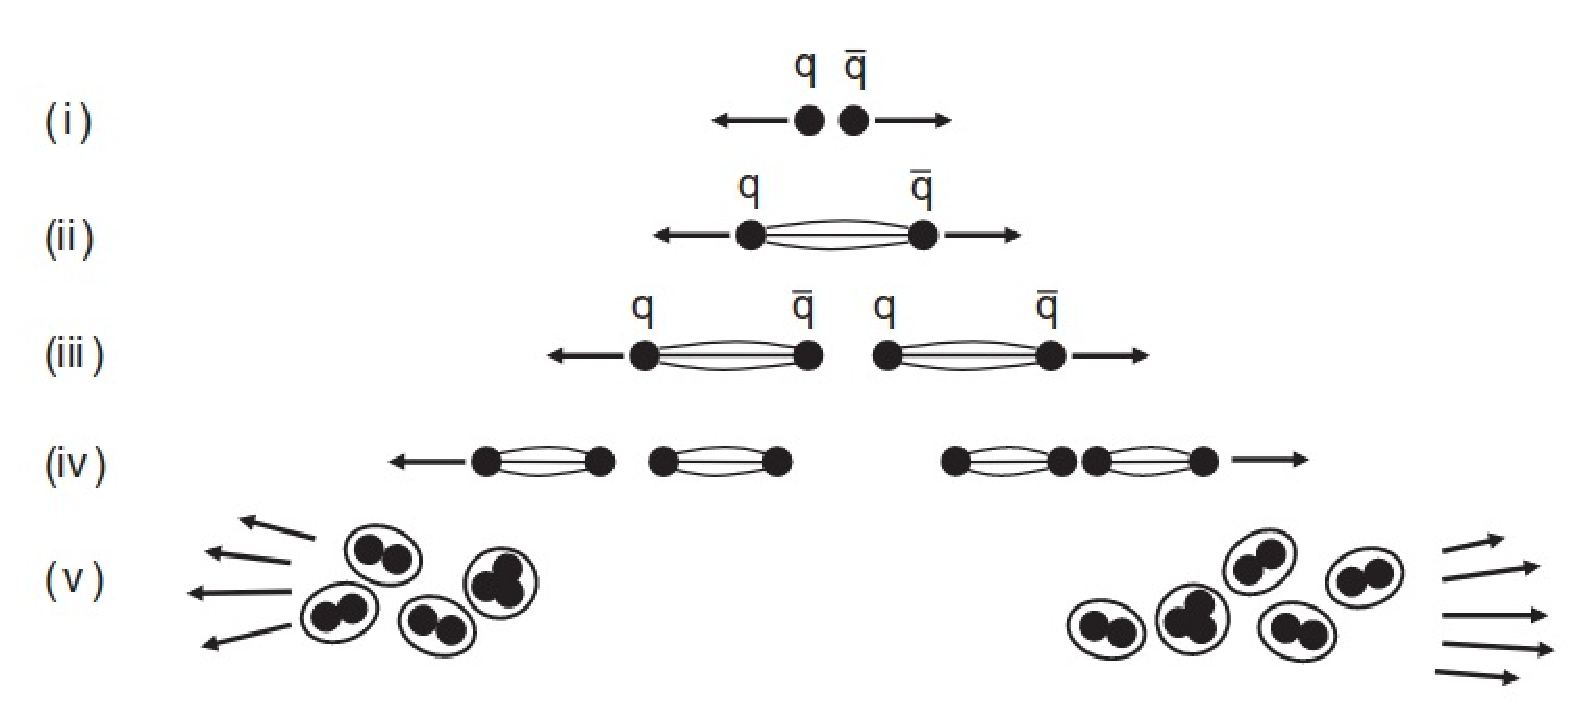
\includegraphics[width=0.9\textwidth]{Figs/Chapter2/Screenshot_20230220_214232.eps}
\end{center}
\caption{Schematic of the quark confinement: (i) the quark and antiquark are pulled away from each other;(ii) as they separated, the string of force tying together the pair stretches; (iii) the energy stored in the string now exceeds the necessary energy for creating a new quark-antiquark pair, the string will break and the two initial quarks will form smaller strings with the newly created pair;(iv) this process continues;(v) until all the quarks and antiquarks have a sufficiently low energy to form hadrons. Figure taken from \cite{thomsonModernParticlePhysics2013}.}
\label{fig:QuarkFragmentation}
\end{figure}

%On another note, hadrons can be classified as a function of their mass hierarchy of their quark constituent with respect to \LambdaQCD:
%\begin{itemize}
%\item[$\bullet$] Any hadron composed exclusively of up, down and strange valence quarks belongs to the \textit{light-flavour sector} ($\Lambda_{QCD} \gg m_{s}, m_{u}, m_{d}$)
%\item[$\bullet$] Any hadron containing, at least, one charm, bottom or top valence quark are members of the \textit{heavy-flavour sector} ($m_{t}, m_{b}, m_{c} \gg \Lambda_{QCD} $)
%\end{itemize}

\subsubsection{Chiral symmetry breaking}
\label{subsubsec:chiralsymmetrybreaking}

In \eq\ref{eq:LagrangianQCD}, the Lagrangian density of QCD was presented and split into four different terms. The quark and gluon kinetic energy and the quark-gluon interaction terms preserve the chiral symmetry, meaning that they leave the chirality of the quarks unchanged. The mass term, though, mixes the left- and right-handed particles:
\begin{equation}
m_{q} \bar{\psi}_{q}^{i} \psi_{qi} = m_{q} \left( \bar{\psi}_{q}^{i, L} \psi_{qi}^{R} + \bar{\psi}_{q}^{i, R} \psi_{qi}^{L} \right).
\label{eq:LagrangianQCDMassTerm}
\end{equation}

The quark mass, $m_{q}$, controls whether the chiral symmetry is broken or preserved. For massless quarks, this term is null hence left- and right-handed particles do not interact together; they would live, somehow, in two separate worlds. Consequently, every hadron would have a twin, identical in every point apart from the handedness: one  is left-handed, the other right-handed. In practice, the quarks have a finite mass but, for the light-flavour ones, it is sufficiently small to consider the chiral symmetry as an approximate symmetry. Therefore, chiral partners are expected to have slightly different masses. However, this is clearly not the case of the $\rho$ ($m_{\rho} = 770 \mmass$) and $a_{1}$ ($m_{a_{1}} = 1260 \mmass$) mesons, meaning that the chiral symmetry is much more broken than expected \cite{kochAspectsChiralSymmetry1997}. 

To be exact, it is \textit{spontaneously} broken\footnote{Well, it is also \textit{explicitly} broken but we will pass on that detail.}. This concept is visualised in \fig\ref{fig:ChiralSymmetryBreaking}. Returning to the example in the note \ref{footnote:SpontaneousSymmetryBreaking}, the continuous transition of the ferromagnet is characterised by an order parameter: the magnetisation. When the temperature is so high that the thermal motions disrupt the alignement of all the magnetic dipoles, the potential is symmetric and the minimum is centred at zero magnetisation (left \fig~\ref{fig:ChiralSymmetryBreaking}). As the temperature decreases and the magnet cools down, the symmetry of the potential is preserved but there are now two minima. The system (the ball) has to choose one, acquiring a non-zero magnetisation in the process, and hence breaking the symmetry (right \figs~\ref{fig:ChiralSymmetryBreaking}). 

\begin{figure}[h]
	\centering
	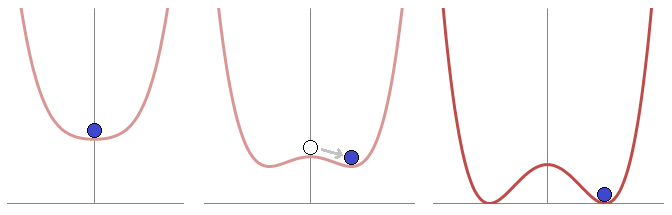
\includegraphics[width=\textwidth]{Figs/Chapter2/Spontaneous_symmetry_breaking_(explanatory_diagram).png}
	\caption{The left figure represents the shape of the potential at high energy, there is one minimum and it is centred on zero. Right figures: as the energy decreases and below a certain critical temperature, the ground state is no longer centred on zero but some distance away from it. Both ground states are equivalent, the system chooses one of them; this is a spontaneous symmetry breaking. The $x$-axis here represents the order parameter. Figure taken from \cite{ft2EnglishExplanatoryDiagram2012}.}
	\label{fig:ChiralSymmetryBreaking}
\end{figure}

The same process occurs for the chiral symmetry but, in this case, the order parameter is the \textit{chiral condensate}. This quantity, $< \psi_{q} \bar{\psi}_{q} > $ or $ < q \bar{q} >$, measures the coupling between left- and right-handed particles in vacuum. It was mentioned earlier that, in QFT, the vacuum is not empty but is composed of fleeting particle-antiparticle pairs that pop in and out. It could be that the Lagrangian density of QCD have an approximate chiral symmetry, but the vacuum does not. This means that particles with different handedness in the vacuum may (or not) interact together, depending the vacuum expectation value of the chiral condensate. If the $ < q \bar{q} >$ is null, the chiral symmetry is restored (left figure~\ref{fig:ChiralSymmetryBreaking}). Conversely, it is spontaneously violated when the chiral condensate is non-zero (right figures~\ref{fig:ChiralSymmetryBreaking}).

This symmetry was extensively studied by Yoichiro Nambu and Giovanni Jona-Lasinio in 1961 \cite{nambuDynamicalModelElementary1961}. In their model, the chiral condensate emerges from the passage of particles in the vacuum\footnote{In fact, the chiral condensate, and hence the spontaneous chiral symmetry breaking, is a consequence of the colour confinement \cite{peskinIntroductionQuantumField2018}.}; for that reason, the chiral symmetry breaking is qualified as \textit{dynamical}. Moreover, as the partons (inside a hadron) travel through the vacuum, they interact with the condensate and acquire an additionnal mass, the \textit{dynamical mass}\footnote{As opposed to the \textit{bare mass} stemming from the Higgs mechanism. It should be mentioned that nothing prevents the gluons to acquire also a dynamical mass. In this case, there would not be massless anymore.}. Predominant fraction of the hadron mass originates from this extra mass: for example, the proton mass sits $\sim 938$ \mmass and the bare mass of its quark constituents represents almost 10 \mmass, that is $\sim $ 1\% of proton mass.\\

On a side note, lattice QCD calculations predict that the chiral symmetry can be restored by heating or compressing matter. This is clear on \fig\ref{fig:ChiralSymmetryBreaking} where the chiral condensate vanishes as the temperature and/or density increases. In such conditions, the ordinary hadronic matter undergoes a phase transition, in which hadrons are only clothed by the bare mass of its constituents.

\begin{figure}[h]
\subfigure[]{
	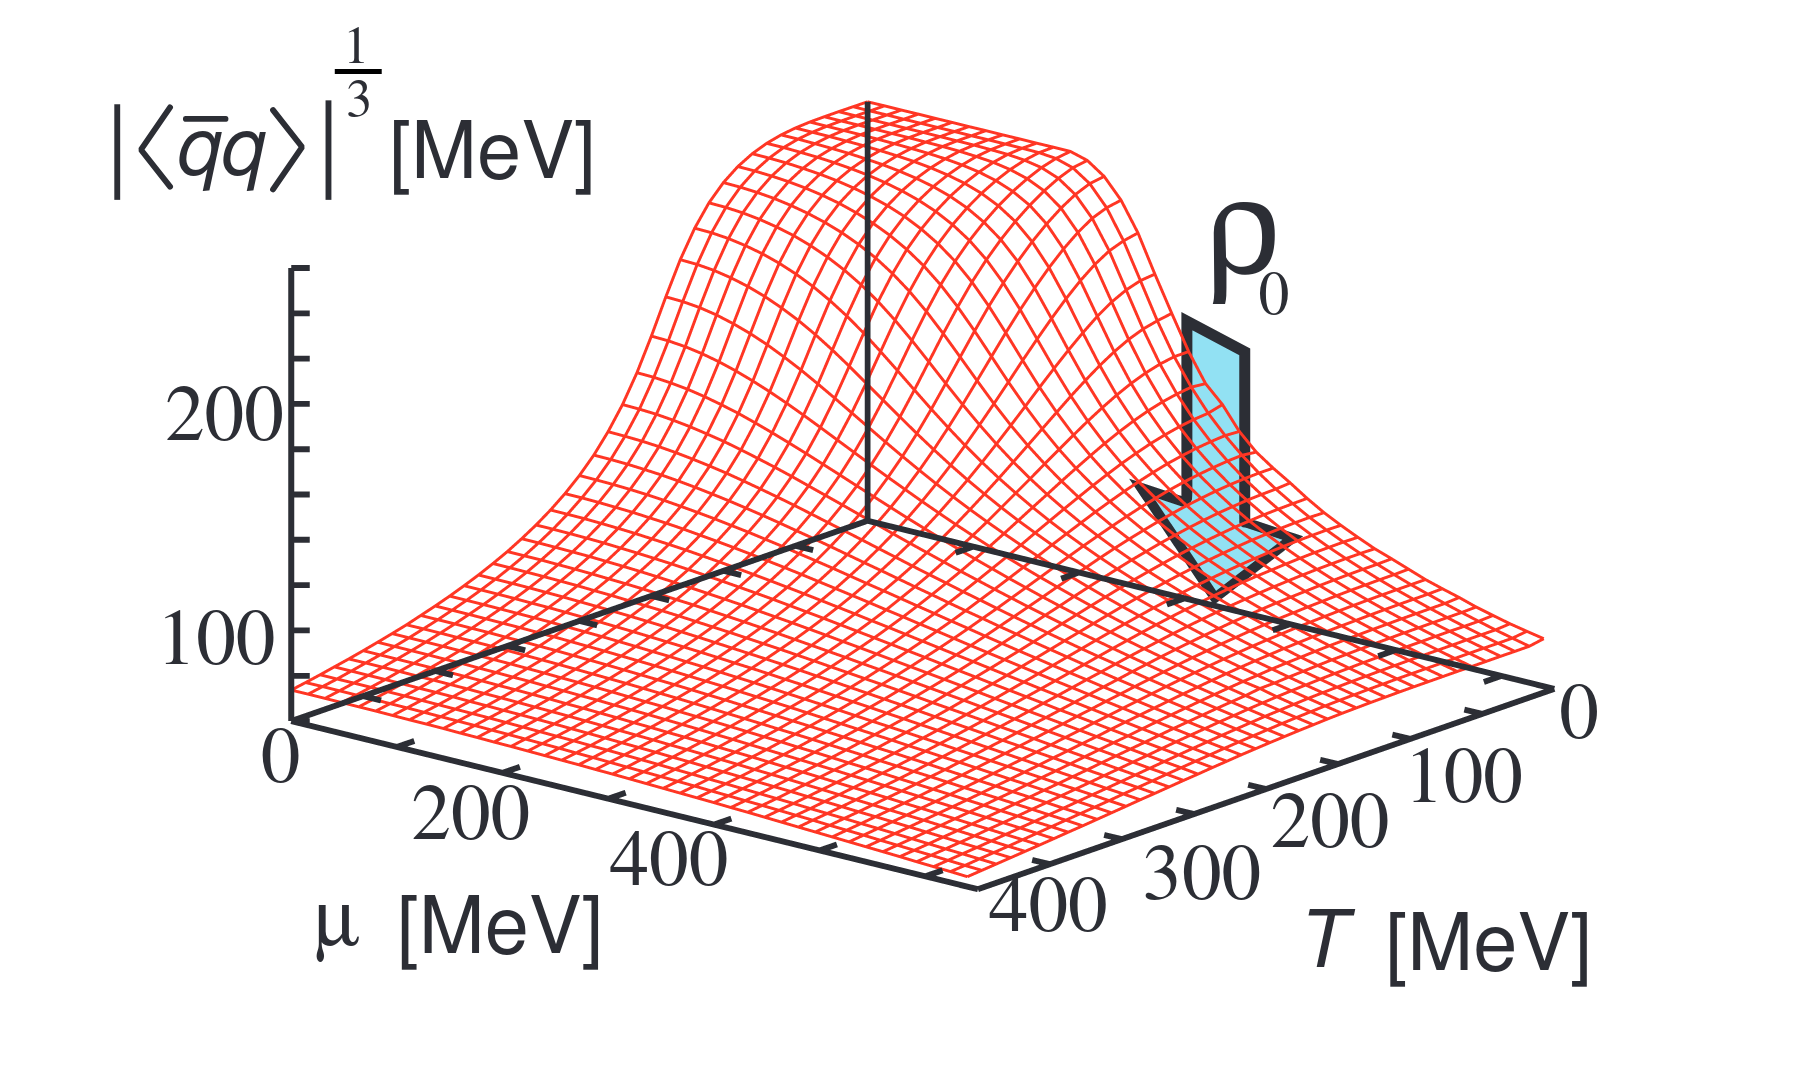
\includegraphics[width=0.50\textwidth]{Figs/Chapter2/ChiralCondensate.png}
}
\subfigure[]{
	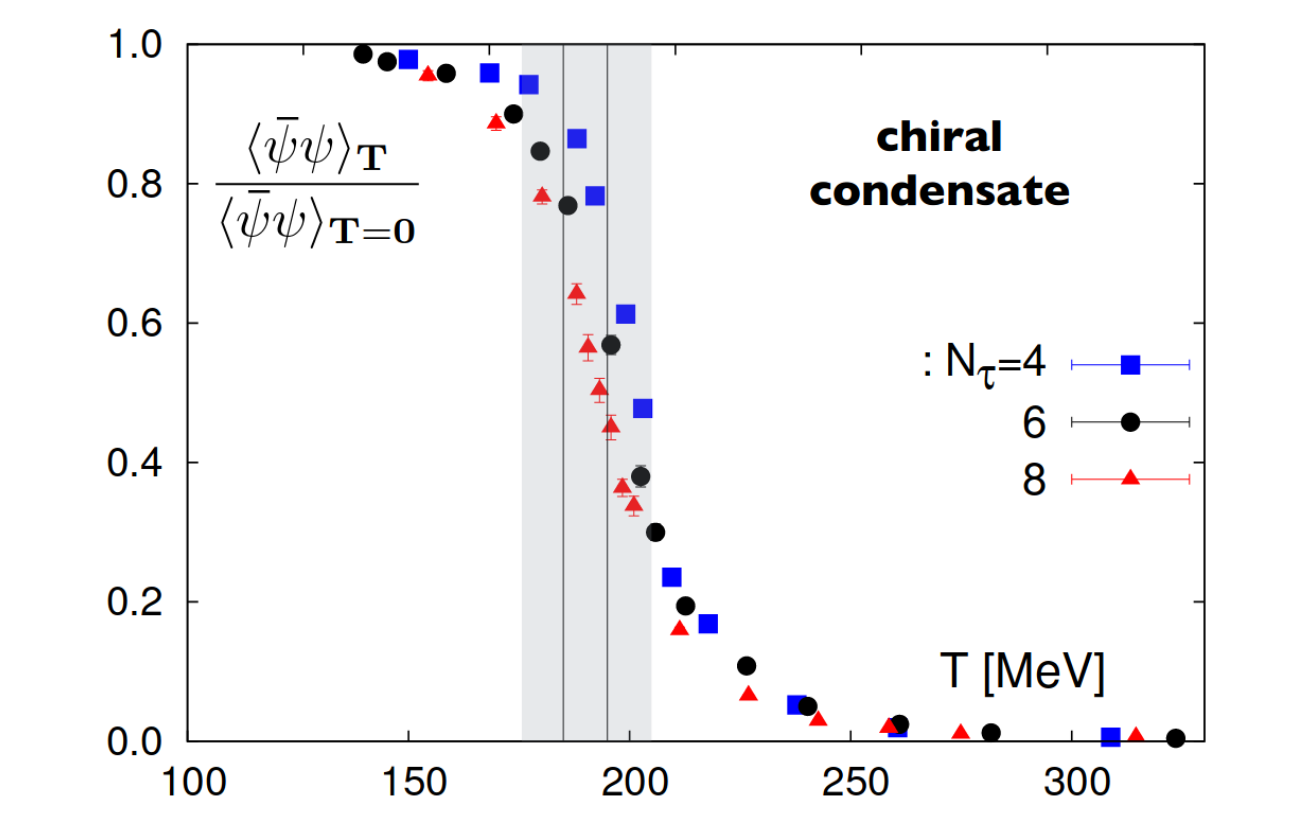
\includegraphics[width=0.50\textwidth]{Figs/Chapter2/ChiralCondensate2.png}
}
	\caption{Lattice QCD results on the evolution of the chiral condensate as a function of (a): the matter density (or the baryochemical potential $\mu$) and the temperature ($T$) \cite{muroyaLatticeQCDFinite2003}, (b): the temperature for different lattice points $N_{\tau}$ \cite{weiseChiralSymmetryStrongly2010}. The arrow on the left figure indicates the value of $\mu$ corresponding the ordinar nuclear density, $\rho_0$. The grey bands on the right figure indicate a range for the transition temperature.}
	\label{fig:ChiralSymmetryBreaking}
\end{figure}

\subsubsection{The QCD-phase diagram}
\label{subsubsec:QCDphasediagram}

In addition to the chiral phase transition, another one comes onto stage as the temperature increases. The \fig\ref{fig:QCDEnergyDensity} shows the predicted evolution of the pressure, energy density and entropy density for a hadron gas as a function of the temperature of the medium. The properties of the gas change rapidly when the temperature reaches $T_{c} = 154$ \mev, indicating the liberation of many degrees of freedom. In this case, these are the partons -- ordinarly confined within hadrons -- that now undergoes a \textit{deconfinement} transition and becomes quasi-free. 

I write \textit{quasi}-free because even at $T \sim 400 $ \mev, the energy density does not reach the ideal gas limit. As a consequence, the quarks and gluons are still interacting but weakly. Due to this shared similarity with the plasmas, this new state of hadronic matter is dubbed \textit{quark-gluon plasma} (QGP). Note that, because the coupling between the partons decreases with the increasing momentum transfer and temperature (asymptotic freedom), the energy density will ultimately overlap with the ideal gas limit but at much larger temperature though. \\

\begin{figure}[h]
	\centering
	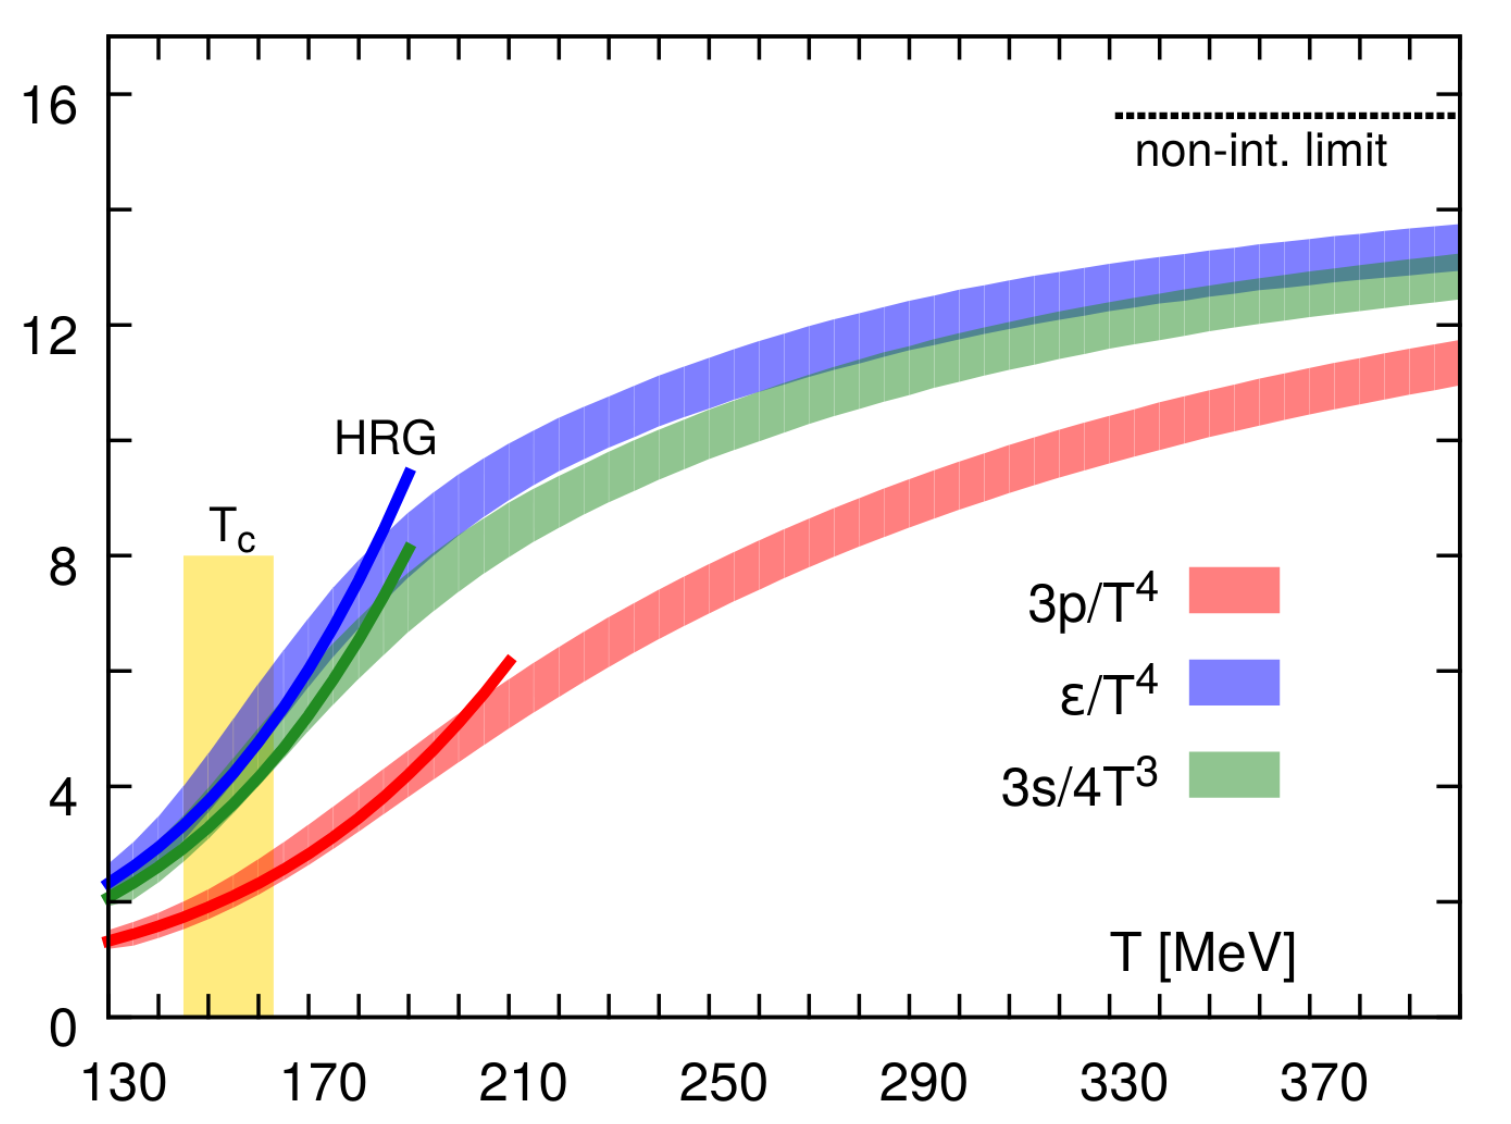
\includegraphics[width=0.7\textwidth]{Figs/Chapter2/Pressure_energy_entropy.png}
	\caption{Lattice QCD calculations of the pressure ($p$), energy density ($\epsilon$) and entropy density ($s$) normalised to the fourth (third, for the last quantity) power of temperature. The solid lines represent the prediction of the hadron resonance gas (HRG) model, the black dashed line indicates the energy density in the limit of an ideal gas. The transition temperature $T_{c}$ is equal to $154 \pm 9$ \mev. It should be emphasised that these predictions have been obtained assuming a zero net baryon density. Figure taken from \cite{bazavovEquationStateFlavor2014}.}
	\label{fig:QCDEnergyDensity}
\end{figure}

The \fig\ref{fig:QCDPhaseDiagram} provides the full QCD phase diagram. As it can be seen, there are two general ways to form a quark-gluon plasma: either one increases the temperature, or one increases the net baryonic density by compressing hadronic matter. The above phase transition corresponds to the former: by heating up the system at (almost) zero net baryon density, ordinary nuclear matter transforms first into a hadron gas and then undergoes a phase transition towards a QGP. This is what someone would see if he/she could rewind the videotape of the time-evolution of the Universe, from nowadays to a few \musec after the Big Bang. In the latter, the ordinary nuclear matter at relatively low temperature acquires, by compression, a larger and larger baryon density until the system transforms into a QGP. This state of matter is supposed to be present in the core of neutron stars\cite{annalaEvidenceQuarkmatterCores2019}, with potentially a colour superconductor behaviour \cite{alfordQCDFiniteBaryon1998}.

\begin{figure}[h]
	\centering
	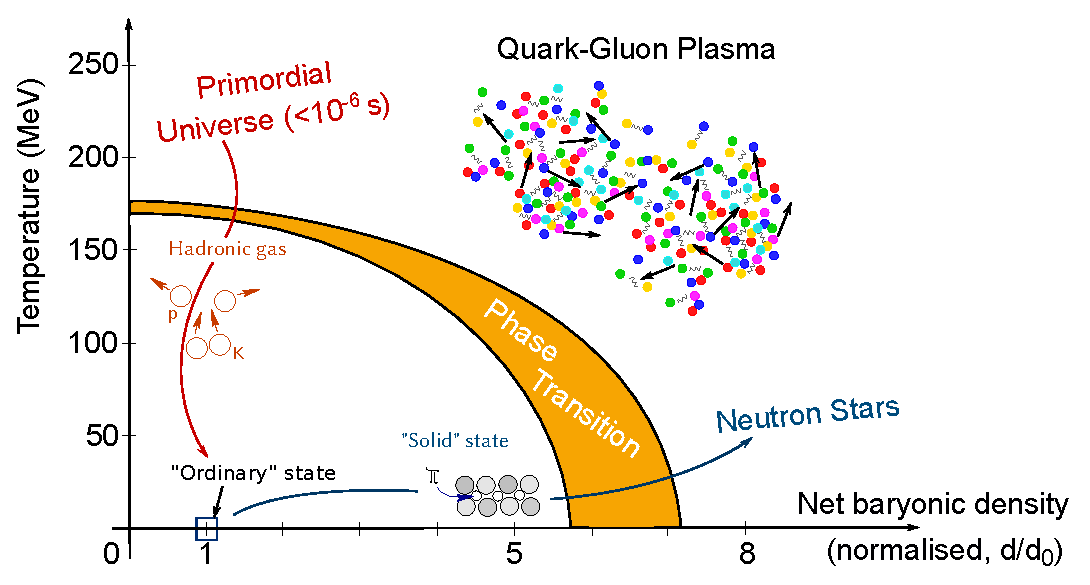
\includegraphics[width=\textwidth]{Figs/Chapter2/DiagrPhase.eps}
	\caption{Schematic representation of the QCD phase diagram as a function of the temperature and the net baryonic density. The latter is normalised to the net baryon density of ordinary nuclear matter. Figure taken from \cite{mairePhaseDiagramQCD2015}.}
	\label{fig:QCDPhaseDiagram}
\end{figure}

There is a profund difference in the nature of the phase transition between the one in the high-temperature region and the other with a high baryon density. Similarly to chiral transition on \fig\ref{fig:ChiralSymmetryBreaking}, the \fig\ref{fig:QCDEnergyDensity} shows a smooth evolution from one phase to another, indicating a second order --- or at least, a crossover --- phase transition \cite{philipsenQCDEquationState2013}. In contrast, the high baryon density driven evolution is expected to be more abrupt, more sharp as when ice melts to turn into water. This corresponds to a first order transition. It follows that there must be a critical point somewhere in the middle of the phase diagram, joining the first and second (or crossover) phase transitions \cite{stephanovQCDPhaseDiagram2005}. Its precise location is currently unknown, as no singularities have been observed yet.


\section{The Quark-Gluon Plasma}
\label{sec:QGP}

Each field of research has its pioneers and the study of the quark-gluon plasma is no exception. The first one was arguably Rolf Hagedorn, who approached the particle production making use of statistical physics. This endeavor led ultimately to the invention of the statistical bootstrap model (SBM) in 1964. At that time, a large number of massive resonances were observed, and this model provided a successful production mechanism for these particles\footnote{The statistical bootstrap model considers a gas of interacting hadrons, composed of all possible particles and their resonances, in a heat bath. If several light hadrons and/or resonances get compressed into a smaller volume, they could themselves be considered as a highly excited and massive resonance (also called fireball). Thus, the hadron gas rather corresponds to a gas of fireballs, that can also become a fireball in itself if compressed. This description provided an explanation for the mass spectrum of hadronic states.}. However, this description was conceived before the development of the quark model. When the quarks were finally considered as the elementary building blocks of hadrons, an extension of SBM was called for \cite{rafelskiMeltingHadronsBoiling2015a}.

The mutation of the statistical hadronisation model was achieved by the father of SBM and Johann Rafelski, between 1977 and 1980. This process led to a new paradigm. It was realised that, at a certain temperature, hadrons are melting to form a new phase composed of boiling quarks: the quark-gluon plasma. Although this concept was already intuited before by numerous physicists -- including Peter Carruthers in 1974 \cite{rafelskiMeltingHadronsBoiling2015} or George F. Chapline and Arthur K. Kerman in 1978 \cite{chaplinePossibilityMakingQuark1978} --, it was only approached qualitatively.

Nevertheless, Chapline and Kerman were the first ones to make the connection between the QGP and (relativistic) heavy-ion collisions. The same year, this point is addressed quantitatively by Siu A. Chin\cite{chinTransitionHotQuark1978a} and later refined in a paper by James D. Bjorken in 1983 \cite{bjorkenHighlyRelativisticNucleusnucleus1983}. In this renowned publication, Bjorken presents an analytical solution for one-dimensional relativistic hydrodynamics in heavy-ion collisions, as well as the space-time evolution of the QGP at mid-rapidity (\textit{Bjorken scenario}), laying down the foundations for the research programme at CERN.\\

Starting in 1986, a vast number of heavy ion experiments emerges at the CERN's Super Proton Synchrotron (SPS): WA85, NA36, NA35, Helios-2, NA38, WA80, and their future descendants \cite{satzSPSHeavyIon2004}. At first, $^{16}$O and $^{32}$S nuclei were accelerated at 200 \gev (per nucleon) until 1995, when the SPS switched to $^{208}$Pb beams with an energy per nucleon of 158 \gev. In a press conference held in February 2000, CERN reports to have \say{compelling evidence that a new state of matter has been created. The new state of matter found in heavy-ion collisions at the SPS features many of the characteristics of the theoretically predicted quark-gluon plasma} \cite{NewStateMatter2023}. This announcement marks a turning point for QGP research: partonic matter is not a mere theoretical concept anymore; it becomes real, tangible and measurable. 

The Relativistic heavy-ion Collider (RHIC) at BNL enters in operation in the next few months, with its four experiments -- BRAHMS \cite{arseneQuarkGluonPlasma2005}, PHOBOS \cite{alPHOBOSPerspectiveDiscoveries2005}, PHENIX \cite{phenixcollaborationFormationDensePartonic2005}, STAR \cite{starcollaborationExperimentalTheoreticalChallenges2005} -- dedicated to observe and characterise the QGP under different observables. In April 2005, BNL holds a press conference in order to present the results of the RHIC experiments, and by doing so, confirms the existence of "a new type of nuclear matter" \cite{ludlamHUNTINGQUARKGLUON2005}.

Nowadays, the study of the QGP is mainly centred around two accelerators: the RHIC at BNL and, since 2009, the Large Hadron Collider (LHC) at CERN. Alike RHIC, the latter also has four experiments: ATLAS, CMS, LHCb and ALICE. Although, they all have a heavy-ion research programme, ALICE is specifically designed to analyse the QGP. Concretely, it pursues the exploration of the QCD phase diagram and the characterisation of this new state of matter initiated at the RHIC, but at much higher energies. For comparison, the LHC delivers Pb-Pb collisions at a centre-of-mass energy per nucleon \sqrtSnn = 2.76 and 5.02 \tev, and Xe-Xe collisions at \sqrtSnn = 5.44 \tev. This is, at least, twenty times more energetic than at the RHIC. The LHC accelerator, as well as the ALICE collaboration, are presented in the next chapter, \chap\ref{chap:ALICE}. 


\subsection{The time evolution of a heavy-ion collision}
\label{subsec:BjorkenScenario}

We timidly started above to raise the question of how a heavy-ion collision leads to the formation of the QGP? This point was addressed by Bjorken in his scenario of the same name. Although the current description turns out to be more complex than anticipated, the Bjorken scenario still provides the key steps of the QGP formation process. The following discussion is structured around the \figs\ref{fig:PbPbSimu} and \ref{fig:QGPEvol}\\

A facility, such as the LHC or RHIC, accelerates heavy nuclei to ultra-relativistic speed. At the LHC energies, the Pb nuclei in each beam are accelerated to, at least, 1.38 \tev\footnote{The least energetic Pb-Pb collision available at the LHC being \sqrtSnn = 2.76 \tev, each beam carries 1.38 \tev per nucleon.}, which corresponds to a Lorentz factor $\gamma$ of about 1500. Consequently, as Bjorken argued \cite{bjorkenHighlyRelativisticNucleusnucleus1983}, even though the partons involved in the collision carry a tiny fraction of the incident beam energy, the nuclei are so extremely boosted that the space-time evolution of the system should be the same in all centre-of-mass frames near central rapidity, and thereby the particle yield should be flat as a function of rapidity, defining a central plateau structure for particle production. Moreover, at such energies, the nuclei are not stopped but rather continue to recede in opposite direction with respect to the collision point; this is the \textit{Bjorken regime} or \textit{transparency regime} and corresponds to net baryonic density close to zero\footnote{As opposed to the \textit{Landau regime} or \textit{stopping regime}, where the nuclei are completely stopped in frontal collisions. It occurs only for collisions at centre-of-mass energies up to a dozen of \gev per nucleon pair. These two regimes actually relates to the two different QGP phase transition: either by heating the system (Bjorken scenario) or compressing it (Landau scenario).}. Another implication is that, because of the length contraction, the nucleus looks like a highly-contracted pancake at mid-rapidity, as can be seen on \fig\ref{fig:PbPbSimu}.\\

\begin{figure}[h]
	\centering
	\hspace*{-2cm}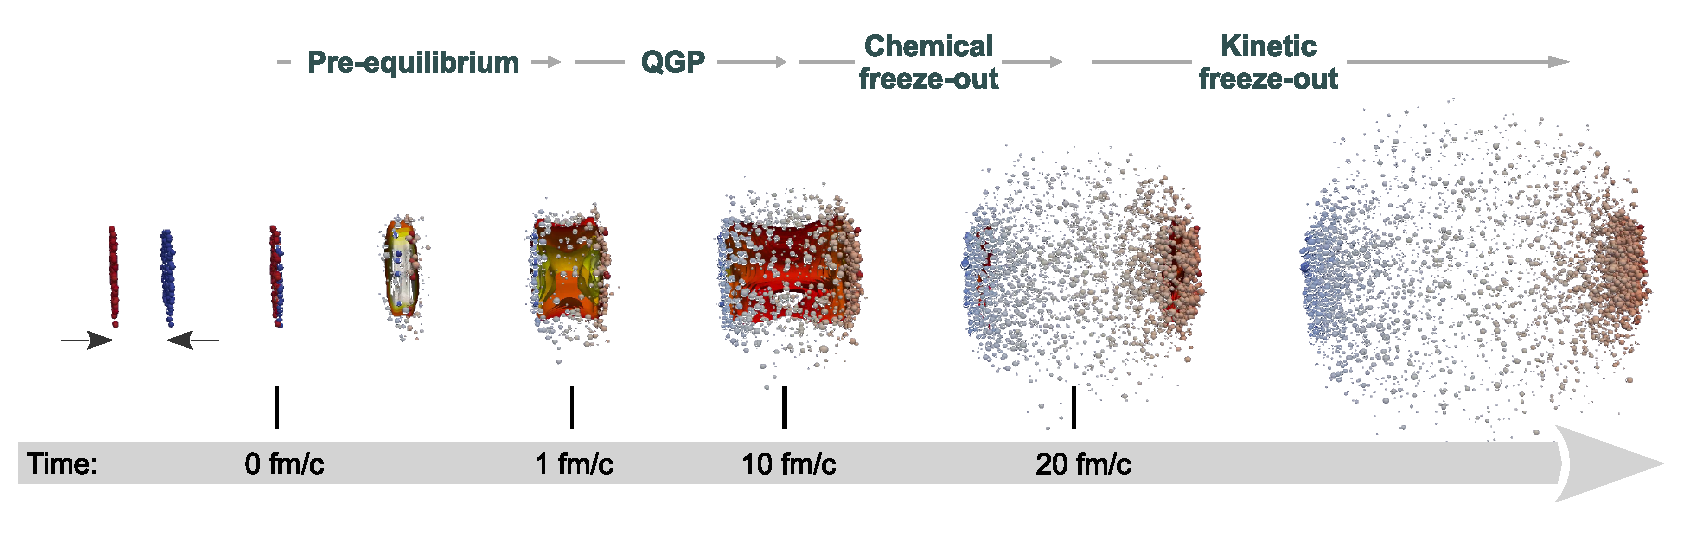
\includegraphics[width=1.35\textwidth]{Figs/Chapter2/PbPbCollision.eps}
	\caption{Simulation of the time evolution of a heavy-ion collision, rendered in seven pictures. Figure originally created by Hannah Petersen, taken from \cite{bernhardBayesianParameterEstimation2018} and modified by the present author.}
	\label{fig:PbPbSimu}
\end{figure}

\begin{figure}[h]
	\centering
	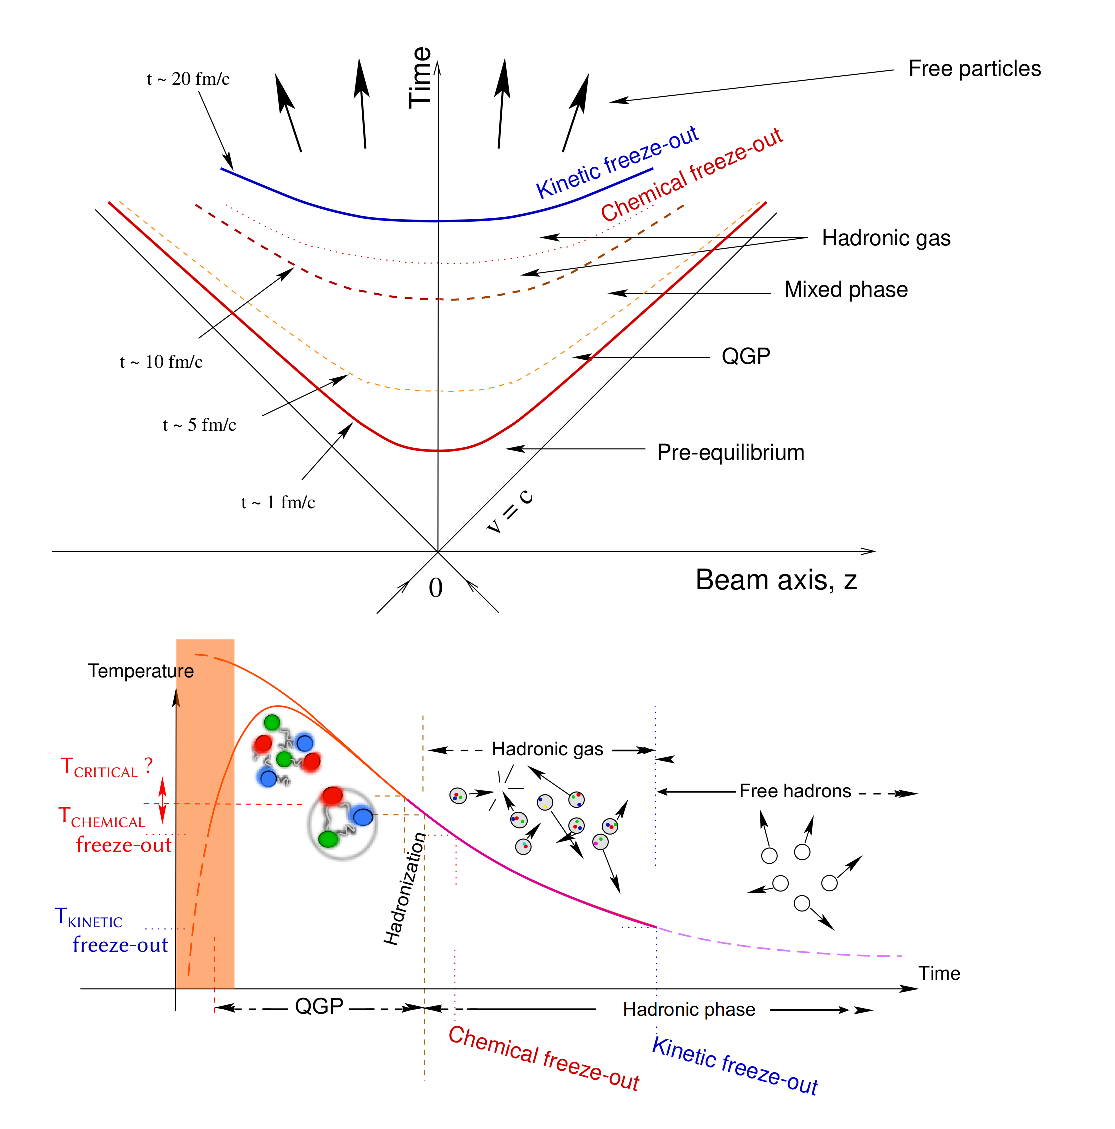
\includegraphics[width=\textwidth]{Figs/Chapter2/Schema-BjorkenScenario.eps}
	\caption{The two views of the Bjorken scenario for ultra-relativistic heavy-ion collisions. Top panel: space-time evolution. Bottom panel: temperature-time evolution. Figure taken from \cite{maireTwoViewsBjorken2011}.}
	\label{fig:QGPEvol}
\end{figure}

The two extremely boosted nuclei approach each other and collide head-on\footnote{Note that this is not necessarily the case, the two nuclei can be slightly shifted. The \textit{impact parameter} quantifies the offset usually in \fm, or alternatively in percentage. In the latter case, we talk about \textit{centrality}. Both parameters are accessible by making use of a \textit{Glauber model}, that provides a semi-classical picture of a nucleus-nucleus collision as a function of the average number of nucleons and nucleon participants in the collision.}. At the same time, the clock associated to the centre-of-mass frame starts to run and indicates 0 \fmC. 

The partons of each nuclei start interacting via either hard-processes -- that involve large momentum transfers and lead to the creation of high momentum partons or massive quarks such as the charm, bottom or even top quarks -- or soft-processes, characterised by small momentum transfer and representing most of the interactions in the initial stage of the collision. As the number of parton-parton interaction increases, the energy density of the system builds up enabling the creation of quarks and gluons out of the vacuum. Rapidly, a dense region of matter (dubbed "fireball") is formed, where partons are strongly coupled but not yet thermalised. This is the pre-equilibrium phase.

Here, the emphasis is on coloured particles, but other kind particles can be produced in the fireball, namely the leptons and photons. Because i) they carry no colour charge and ii) the typical interaction time of the weak ($\approx 10^{-10} \sec$) and electromagnetic forces ($\approx 10^{-16} \sec$) is too short compared to the timescale of a heavy-ion collision ($\approx 10^{-23} \sec$), they will simply escape the medium unaffected.

%\footnote{Here, the emphasis is on coloured particles, but other kind particles can materialise out of the vacuum, namely the leptons. Because i) they carry no colour charge and ii) the typical interaction time of the weak ($\approx 10^{-10} \sec$) and electromagnetic forces ($\approx 10^{-16} \sec$) is too short compared to the timescale of a heavy-ion collision ($\approx 10^{-23} \sec$), they will simply escape the collision environment.}


If the energy density is high enough (typically around 1 \gev/\fm$^{3}$), the initially produced matter undergoes, first, a phase transition towards the restoration of the chiral symmetry and, if possible, then towards the QGP. Due to multiple interaction between the medium constitutents, the energy gets distributed evenly among them leading the system to a thermal equilibrium around 1 \fmC ($\approx 10^{-23} \sec$) after the collision\footnote{Note that this is not a mandatory step for the QGP formation.}. 

Once the QGP is formed, it experiences two expansions. Driven by the non-uniform geometrical energy distribution in the initial stage of the collision, a pressure gradient appears in the QGP, which results in a radial expansion of the system. Furthermore, the boost of the two incident nuclei causes the plasma of quarks and gluons to inflate in the longitudinal directions. Since the energy deposited initially in the system is fixed and its spatial size keeps extending, the energy density decreases and inevitably, the fireball cools down.\\

At some point, most of the parts of the system goes below the critical temperature, the deconfined partons start to recombine into hadrons. The QGP evaporates into a gas of hadrons. Note, that because the chiral transition -- in this case, from a restored symmetry to a broken one -- occurs below $T_{c}$, the mesons and baryons formed during this hadronisation process only carry the bare mass of their constituents. At least, until the system further cools down and undergoes a phase transition towards a breaking of the chiral symmetry, as explained in the \Sec\ref{subsubsec:chiralsymmetrybreaking}.

The energy density within the hadron gas remains significant, sufficiently to allow for inelastic collisions. Consequently, the chemical composition in terms of particle species is in constant evolution. Around 10 \fmC, as the energy density decreases, inelastic interactions become less and less frequent. They become impossible when the gas reaches the \textit{chemical freeze-out} temperature. The particle composition is now fixed but hadrons can still interact elastically.\\

Although, the hadron content should be fixed, some resonances can still regenerate via pseudo-elastic scattering. This is, for example, the case of the \rmKstarZero that can be recreated through \rmPiPM-\Kminplus interaction. On the other hand, elastic scatterings modify the momentum of one of its decay products. In such a case, the measured yield would decrease.  

At 20 \fmC, the hadron gas fades into free hadrons. The momenta of the hadrons are now fixed. This is the \textit{kinetic freeze-out}. These particles will fly towards the detectors and, for some of them, decay via weak or electromagnetic interactions. Either the particles originate directly from the collision or are decay products, once they have reached the detector, they will be detected and reconstructed, giving rise to an event such as the one displayed in the \fig\ref{fig:ALICEEventDisplay}.

\begin{figure}[h]
	\centering
	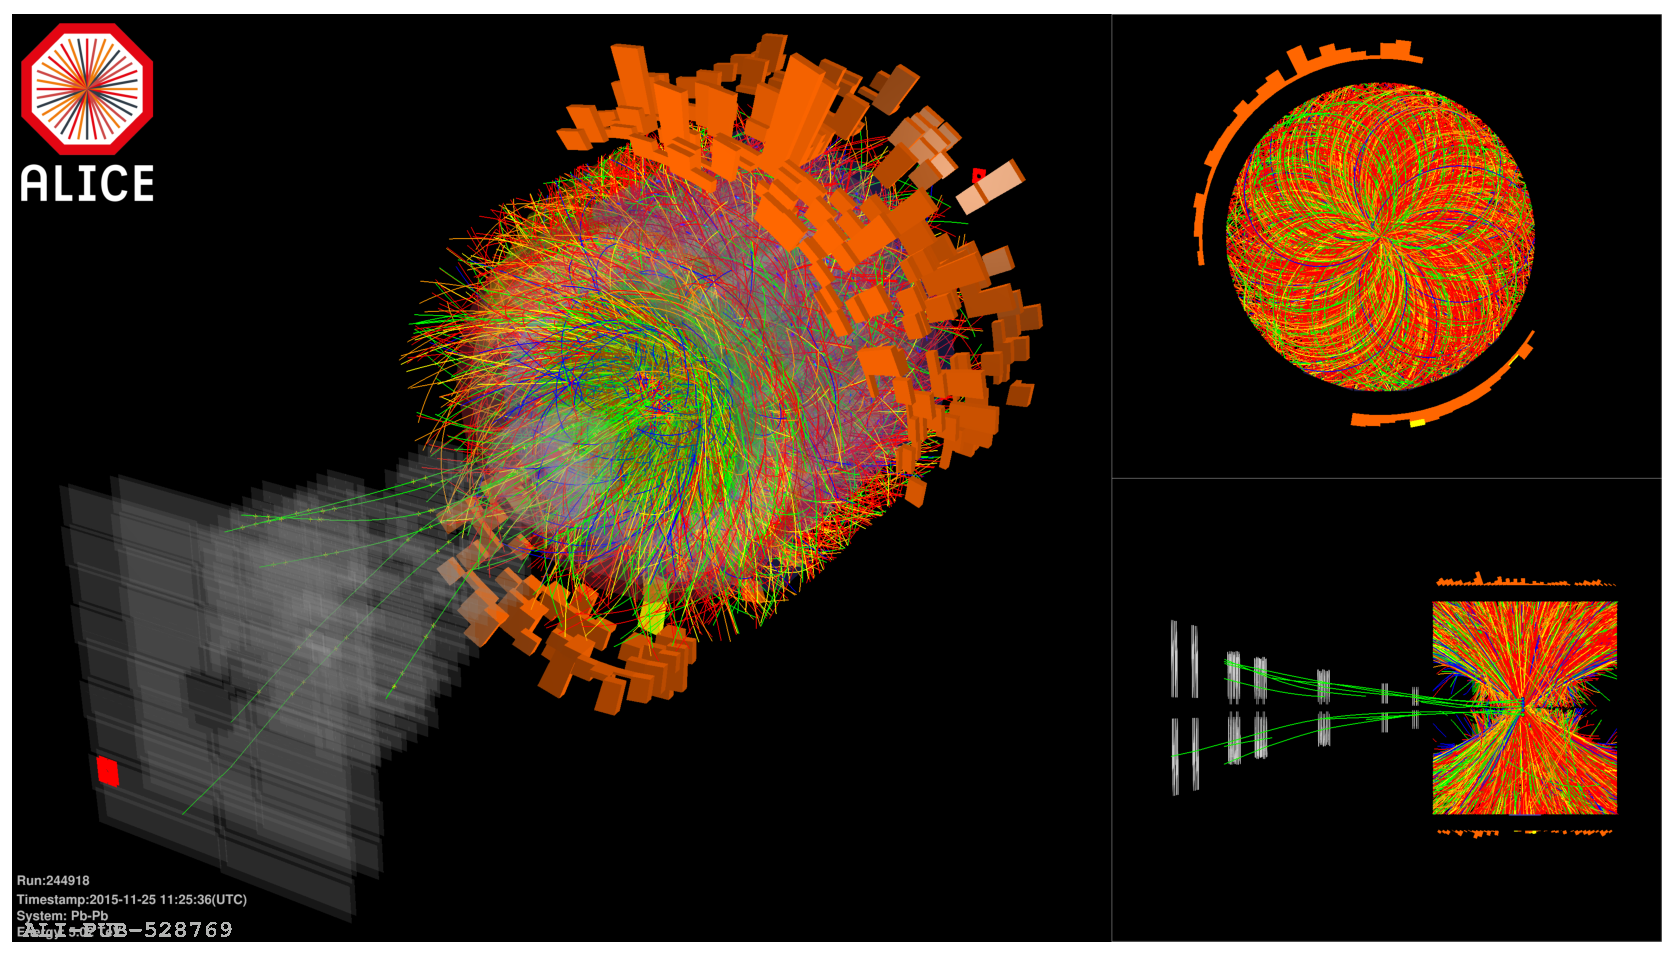
\includegraphics[width=\textwidth]{Figs/Chapter2/ALICE_EventDisplay.eps}
	\caption{Event display of the particles reconstructed with the ALICE detector and created in a Pb-Pb collision at \sqrtSnn = 5.02 \tev in 2015. Figure taken from \cite{alicecollaborationALICEExperimentJourney2022}.}
	\label{fig:ALICEEventDisplay}
\end{figure}

In total, the QGP only exists for about $10^{-22}\sec$, which is currently impossible to reach for the most advanced readout electronics. The study of this state of matter relies on the signatures that are printed in the detectors after the collision. Theoretical models provide predictions of what the QGP footprints look like. Nowadays, it is widely admitted that the following signatures are marks of the QGP.

\begin{itemize}
\item[$\bullet$] \textbf{Collective flow:} The QGP being an almost perfect liquid of constituents with small mean free path, the pressure gradient created by the collision leads to a collective flow, \ie flow of partons, that can be described in the final state by ultra-relativistic hydrodynamic models.  This aspect is addressed, in particular, by performing measurements sensitive to the radial/isotropic and anisotropic flow. The former is characterised by a boost of the low-\pT produced hadrons to higher \pT --- the higher the mass, the higher the boost ---; the latter is studied through a Fourier series decomposition of the azimuthal distribution of the emitted particle density. Moreover, the collective motion of partons can also be observed looking at long-range particle correlation.\\

\item[$\bullet$] \textbf{Direct photons:} Photo-production occurs over the entire duration of the collisions, but it is strongly increased when the system is hot. Therefore, a significant excess of \textit{direct}\footnote{The term \textit{direct} aims at designating only the photons originating from the different stage of the collisions (prompt), and not the ones from hadronic decays (non-prompt).} photons is observed in heavy-ion collisions, suggesting that a QGP has been formed there. Moreover, since they leave the medium unaffected, they carry informations on its properties. In particular, the low-\pT photons are essentially produced out of the plasma heat, hence they are designated as \textit{thermal photons}. Accounting for the blue-shift induced by radial expansion of the system (Doppler effect), the measurement of their yield provides an effective temperature of $304 \pm 41$ \mev in the most central Pb-Pb collisions \cite{alicecollaborationALICEExperimentJourney2022}.\\

\item[$\bullet$] \textbf{Jet quenching:} The high-\pT or massive partons are produced in the early stage of the collision. As they interact with other soft partons of the QGP, a part of their energy is transferred to the medium, resulting in energy loss effects. They are of two kinds: collisional, which consists in elastic scattering \textit{with} the medium constituents, and radiative that corresponds to an inelastic interaction and results in the emissions of gluons \textit{within} the QGP. In the case of two jets, back-to-back, created close to the phase boundary, one will escape the fireball whereas the other will loose most of its energy in the medium. Thus, if one of the back-to-back jets is missing in the event, this would suggest the existence of a hot and dense medium, as observed in \cite{alicecollaborationSuppressionChargedParticle2011}\\

%However, the emission angle decreases with the number of emitted gluons, and the probability of radiating a gluon at a given angle depends on the parton mass. In particular for heavy quarks, there exists a cone region wherein there can be any gluon emission. This is called the \textit{dead cone effect}. Because of that, jets originating from a $c$ or $b$ quark will mainly loose energy \\
\item[$\bullet$] \textbf{Heavy quarkonia suppression:} The heavy quarks, such as charm or beauty, can fragment and hadronise to form a quarkonia ($c\bar{c}$ or $b\bar{b}$ mesons). Because of the low binding energy of these states, they will start to melt and dissolve within the medium. On the other hand, this suppression can be counter-balanced by a regeneration of the quarkonia state: at the chemical freeze-out, it is possible for a heavy quark to recombine with a heavy anti-quark. Therefore, the quarkonia production is compared to theoretical models, and so far, the results are consistent with the formation of a QGP.\\

\item[$\bullet$] \textbf{Hadron abundancy:} At chemical freeze-out, the hadron gas is supposed to be in thermal and chemical equilibrium. The hadron composition in the hadron can therefore be addressed in a statistical approach using the grand canonical formalism. The \textit{statistical hadronisation model} (SHM) provides a prediction of the mesons and baryons abundancies, as a function of the gas volume and temperature, and the different chemical potentials ($\mu_{B}$ for the baryonic one, $\mu_{S}$ for the strangeness one,...). By fitting the measured yields of various hadron species with the SHM prediction, the chemical freeze-out temperature $T_{\textrm{ch}}$ and volume $V_{\textrm{ch}}$ can be estimated. The values $T_{\textrm{ch}} = 155 \pm 2 \ \mev$ and $V_{\textrm{ch}} = 5924 \pm 543 \ \fm^{3}$ are consistent with lattice QCD calculations. \\
\end{itemize}

About abundancy, the one of strange particles stands out of the other species. It is, in fact, one of the historical key signatures of the QGP and is called the \textit{strangeness enhancement}. 

\subsection{Strangeness enhancement}
\label{subsec:StrangenessEnhanement}

The concept of strangeness enhancement, that consists in the abundant production of strange hadrons in heavy-ion collisions, starts to take shape in the mind of Johann Rafelski in 1980. The original argument is based on the assumption that, in a melted vacuum such as the one that settles in the QGP pre-equilibrium stage, the chiral symmetry restoration results in strange quarks carrying only their bare mass ($m_{s}$), that is at least two times lower than QGP temperature ($2 m_{s} < T_{\textrm{QGP}}$) . Thus, this opens the way to a chemical equilibration/saturation of strangeness. When the fireball cools down, the numerous $s$ and $\bar{s}$ tend to hadronise into strange baryons ($qqs$ or $\bar{q}\bar{q}\bar{s}$,...) rather than mesons ($\bar{q}s$ or $q\bar{s}$).

Back then, gluons were still hypothetical objects. Strangeness production was mainly considered in the annihilation process of light quark pairs $q\bar{q} \rightarrow s \bar{s}$ (\fig\ref{fig:StrangeYields}d). In 1981, J\'ozsef Zim\'anyi and Tam\'as B\'ir\'o estimated that, with this process, the chemical equilibrium of strangeness takes too much time to settle and is reached around eight times the natural lifespan of a QGP fireball. However, Zim\'anyi and B\'ir\'o assumed that there were no gluons and were focused on the physical case of a hadron gas \cite{rafelskiStrangenessEnhancement2008}.

In parallel, it was realised that gluon fusion processes dominates the production rates. Together with Berndt M\"{u}ller, Rafelski shows in 1982 that the chemical equilibration of strangeness is possible within the QGP lifespan thanks to the fusion of gluons created out of the vacuum heat  \cite{rafelskiStrangenessProductionQuarkGluon1982}. The different $gg \rightarrow s\bar{s}$ processes are depicted in \fig\ref{fig:StrangeYields}a,b,c.

%\begin{figure}[h]
%	\centering
%	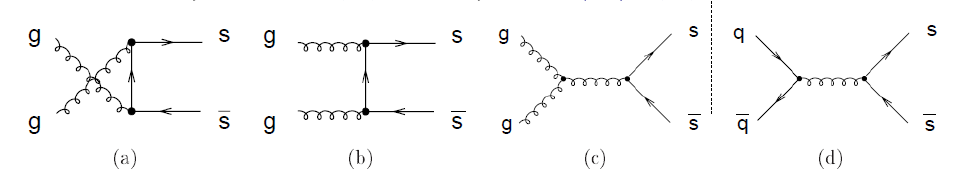
\includegraphics[width=1\textwidth]{Figs/Chapter2/Screenshot_20220620_004959.png}
%	\caption{The lowest-order QCD diagrams for $s\bar{s}$ production. (a)(b)(c) the different gluon fusion processes $gg\rightarrow s\bar{s}$; (d) quark-antiquark annihilation process $q\bar{q} \rightarrow s\bar{s}$. Figure taken from \cite{maireProductionBaryonsMultietranges2011}.}
%	\label{fig:StrangenessEnhancement}
%\end{figure}

\begin{figure}[h]
	\begin{minipage}{0.33\textwidth}
		\subfigure[]{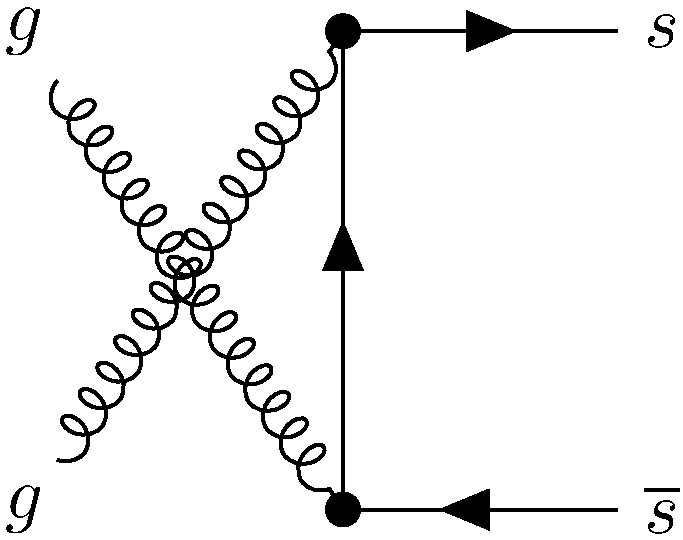
\includegraphics[width=0.75\textwidth]{Figs/Chapter2/g+g_crossed_to_s+sbar.pdf}}
	\end{minipage}%
	\begin{minipage}{0.33\textwidth}
		\subfigure[]{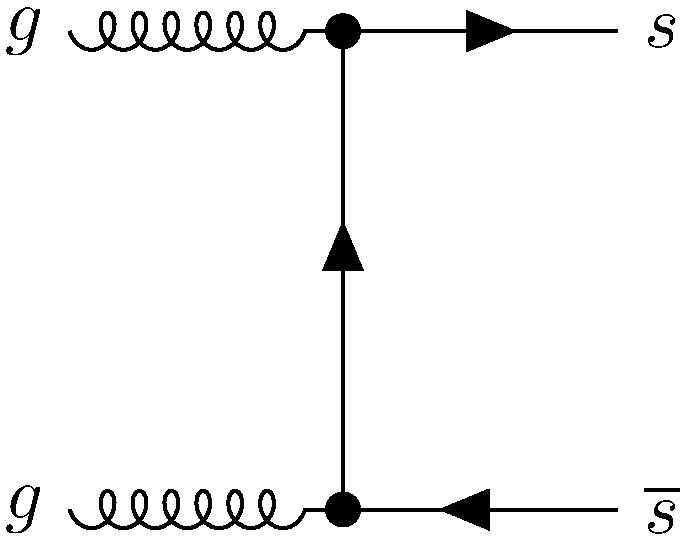
\includegraphics[width=0.75\textwidth]{Figs/Chapter2/g+g_square_to_s+sbar.pdf}}
	\end{minipage}%
	\begin{minipage}{0.33\textwidth}
		\subfigure[]{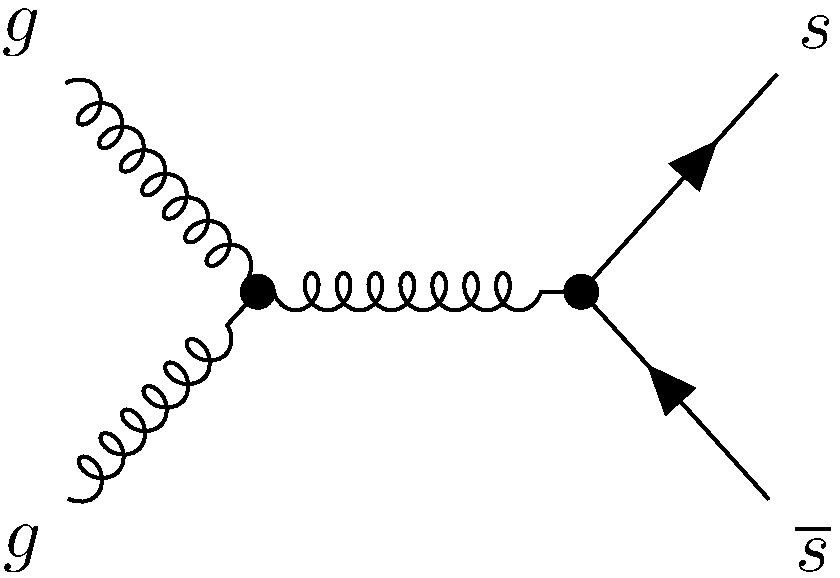
\includegraphics[width=0.90\textwidth]{Figs/Chapter2/g+g_to_gluon_to_s+sbar.pdf}}
	\end{minipage}\par\medskip
	\centering
	\begin{minipage}{0.33\textwidth}
		\subfigure[]{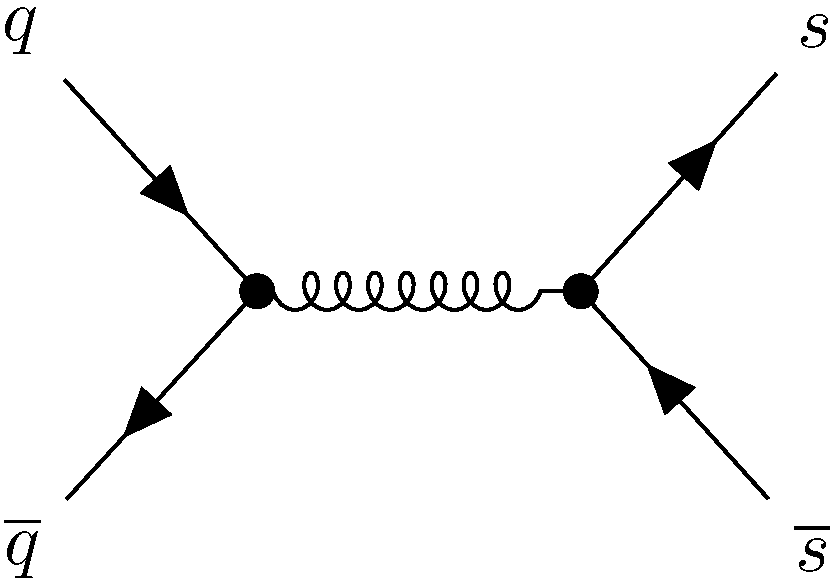
\includegraphics[width=0.90\textwidth]{Figs/Chapter2/q+qbar_to_gluon_to_s+sbar.pdf}}
	\end{minipage}%
	\caption{The lowest-order QCD diagrams for $s\bar{s}$ production. (a)(b)(c) the
	 different gluon fusion processes $gg\rightarrow s\bar{s}$; (d) quark-antiquark annihilation process $q\bar{q} \rightarrow s\bar{s}$. Figure taken from \cite{maireProductionBaryonsMultietranges2011}.}
	\label{fig:StrangenessEnhancement}
\end{figure}



In summary, the strangeness enhancement was proposed by Rafelski and M\"{u}ller in 1982 as a signature of a deconfined quark-gluon matter. They demonstrated that:
\begin{itemize}
\item the QGP begins to be saturated by strange quarks and anti-quarks when the temperature of the plasma reaches the 200 \mev after about $2 \times 10^{-23} \sec$,
\item this saturation is possible because strange quarks can pop in out of the QGP heat ($2 m_{s} < T$) via gluon fusion processes (\fig\ref{fig:StrangenessEnhancement}). These processes are favoured because i) they are more energy/time efficient and ii) the high density of gluons created out of the vacuum,
\item at the hadronisation, the strangeness tends to be distributed on baryons rather than mesons. Consequently, this leads to an increased production of strange particles in the final state of the collision. In fact, the larger the strangeness content, the larger the enhancement of the hadron production.\\
\end{itemize}

Experimentally, the strangeness enhancement manifests itself through an increase of the \textit{relative} yields of strange hadrons in heavy-ion collisions. Now comes two difficulties: so far, only the strangeness enhancement from the formation of a QGP was considered, however a similar phenomenon could occur in a hadron gas\footnote{Strange hadrons could be formed via inelastic collisions between light mesons and baryons. Because of the large dynamical mass of hadrons, the production of strange particles should be suppressed. This reduction gets more pronunced as the hadron mass is high.}. The difference between these two increases in strange particle abundancies resides in the hierarchy between hadrons with different strangeness content \cite{maireProductionBaryonsMultietranges2011}:

\begin{align}
\rmOmega(sss)\ /\ \rmXi(dss) _{\textrm{QGP}} \quad &\approx \quad \rmXi(dss)\ /\ \rmLambda(uds) _{\textrm{QGP}}\\
\rmOmega(sss)\ /\ \rmXi(dss) _{\textrm{Hadron Gas}} \quad &\ll \quad \rmXi(dss)\ /\ \rmLambda(uds) _{\textrm{Hadron Gas}}
\end{align}

\begin{align}
\rmOmega(sss)\ /\ \rmXi(dss) _{\textrm{QGP}} \quad &> \quad \rmOmega(sss)\ /\ \rmXi(dss) _{\textrm{Hadron Gas}}\\
\rmXi(dss)\ /\ \rmLambda(uds) _{\textrm{QGP}} \quad &> \quad \rmXi(dss)\ /\ \rmLambda(uds) _{\textrm{Hadron Gas}}
\end{align}


Another issue arises from the definition of \textit{relative} yields. In other words, this comes down to asking what normalisation to use? There are different possibilities, depending on the physics target. Most of the time, the yields of strange hadrons in heavy-ion collisions are compared to the ones in pp collisions. This is relevant in order to discriminate the strangeness enhancement originating from the QGP (heavy-ion collisions) from the one occuring in a hadron gas (as in pp collisions, assuming that there are enough interactions between the different produced hadrons). Alternatively, one could also look at the "continuous" evolution of the yields as a function of the collision system. In such a case, the relative yields correspond to the ratio of production rate between the particle of interest and the lighest known hadron, namely the \rmPi. Finally, the focus can also be on the difference of yields between hadrons with the same strangeness content but different mass, typically the yields ratio between a resonant and a non-resonant hadronic state. This could provide some information on the influence of the hadronic phase.\\

\begin{figure}[h]
	\centering
	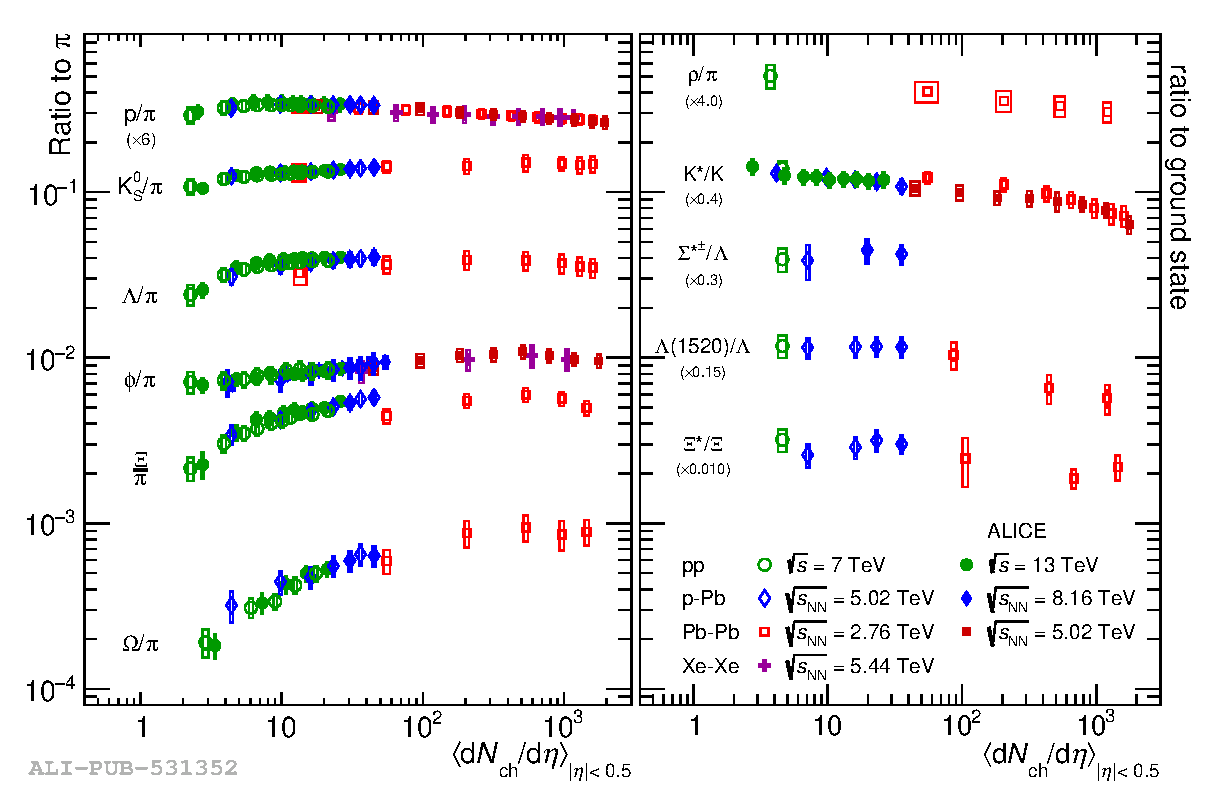
\includegraphics[width=1\textwidth]{Figs/Chapter2/fig3.2a.eps}
	\caption{(Left panel) Relative yields of strange hadrons with respect to the pions and (right panel) yield ratios between resonant and ground state hadrons as a function of the average charged particle multiplicities at midrapidity. Results from different collision systems are presented: pp at \sqrtS = 7 and 13 \tev; p-Pb at \sqrtSnn = 5.02 and 8.16 \tev; Pb-Pb at \sqrtSnn = 2.76 and 5.02 \tev; Xe-Xe at \sqrtSnn = 5.44 \tev. The left panel considers the following strange hadrons: \rmKzero ($\bar{d}s$), \rmLambda ($uds$), \rmPhi ($s\bar{s}$), \rmXi ($dss$) and \rmOmega ($sss$). The error bars corresponds to the statistical uncertainty, whereas the boxes show the total systematic uncertainty. Figure taken from \cite{alicecollaborationALICEExperimentJourney2022}.}
	\label{fig:StrangeYields}
\end{figure}

The \fig\ref{fig:StrangeYields} presents, on the left, the measurement of relative yields of strange hadrons with respect to the pions a function of the average charged multiplicity of the collision, and on the right, the yield ratios between resonant and non-resonant states are displayed. The lowest multiplicities correspond to pp collisions, and as it increases, we move on towards more and more central heavy-ion collisions.

The left panel of \fig\ref{fig:StrangeYields} shows that the yield of strange hadrons increases in Pb-Pb and Xe-Xe collisions with respect to pp and p-Pb collisions, and the enhancement factor gets bigger with the strangeness content. This is compatible with the strangeness enhancement picture and confirms the existence of a deconfined quark-gluon matter. Notice that the ratios do not change with the centre-of-mass energy, suggesting that the initial stage of the collision does not play an important role in the strangeness enhancement (at least, at the LHC energies).

On the right panel, the yield ratios between resonant and non-resonant hadronic states seems to decrease when going from elementary collision systems (pp and p-Pb) to the heavy-ion ones. This trend indicates that the temperature of the hadron gas after the QGP is sufficiently high to suppress the resonance yields by elastic rescattering of the decay products.

%\begin{figure}
%\unitlength = 1mm
%\centering
%\subfigure[]{
%	\begin{fmffile}{ggxss}
%	\begin{fmfgraph*}(40,25)
%	\fmfleft{i1,i2}
%	\fmfright{o1,o2}
%	\fmflabel{$g$}{i1}
%	\fmflabel{$g$}{i2}
%%	\fmflabel{$s$}{o1}
%%	\fmflabel{$\bar{s}$}{o2}
% 	\fmf{fermion}{o1,v1}
% 	\fmf{fermion,tension=0}{v1,v2}
% 	\fmf{fermion}{v2,o2}
% 	\fmffreeze
%	\fmf{gluon}{i1,v1}
%	\fmf{gluon,rubout}{i2,v2}
%%    \fmf{fermion}{i1,v1,v2,o1}
%%	\fmf{fermion}{o2,v4,v3,i2}
%%	\fmf{photon,tension=0}{v1,v3}
%%	\fmf{photon,tension=0}{v2,v4}
%	\end{fmfgraph*}
%	\end{fmffile}
%}
%\subfigure[]{
%	\begin{fmffile}{gghss}
%	\begin{fmfgraph*}(35,25)
%	\fmfleft{i1,i2}
%	\fmfright{o1}
%	\fmflabel{$g$}{i1}
%	\fmflabel{$g$}{i2}
%	\fmflabel{$g$}{o1}
%	\fmf{gluon}{i1,v1}
%	\fmf{gluon}{i2,v1}
%	\fmf{gluon}{v1,o1}
%	\fmfv{lab=$g_s$,lab.dist=0.15w}{v1}
%	\fmfdot{v1}
%	\end{fmfgraph*}
%	\end{fmffile}
%}
%\subfigure[]{
%	\begin{fmffile}{ggss}
%	\begin{fmfgraph*}(40,25)
%	\fmfleft{i1,i2}
%	\fmfright{o1,o2}
%	\fmflabel{$g$}{i1}
%	\fmflabel{$g$}{i2}
%	\fmflabel{$s$}{o1}
%	\fmflabel{$\bar{s}$}{o2}
%	\fmf{gluon}{i1,v1}
%	\fmf{gluon}{v1,i2}
%	\fmf{fermion}{v2,o1}
%	\fmf{fermion}{o2,v2}
%	\fmf{gluon}{v1,v2}
%	\fmfdot{v1}
%	\fmfdot{v2}
%	\end{fmfgraph*}
%	\end{fmffile}
%}
%\subfigure[]{
%	\begin{fmffile}{qqss}
%	\begin{fmfgraph*}(40,25)
%	\fmfleft{i1,i2}
%	\fmfright{o1,o2}
%	\fmflabel{$q$}{i1}
%	\fmflabel{$\bar{q}$}{i2}
%	\fmflabel{$s$}{o1}
%	\fmflabel{$\bar{s}$}{o2}
%	\fmf{fermion}{i1,v1}
%	\fmf{fermion}{v1,i2}
%	\fmf{fermion}{v2,o1}
%	\fmf{fermion}{o2,v2}
%	\fmf{gluon}{v1,v2}
%	\fmfdot{v1}
%	\fmfdot{v2}
%	\end{fmfgraph*}
%	\end{fmffile}
%}
%\caption{Using \texttt{test}}
%\end{figure}

\subsection{Comparison with elementary systems}
\label{subsec:ComparisonPP}

Throughout this section, it was suggested that the formation of the QGP is exclusive to heavy-ion collisions, and it is not expected in more elementary systems -- such as pp and p-Pb collisions -- because the size of the colliding system is \textit{a priori} too small. Looking more attentively at the \fig\ref{fig:StrangeYields}, one notices that relative yields of strange hadrons increases smoothly from low to high multiplicity pp and p-Pb collisions. In other words, this means that strangeness enhancement seems to be present as well in small systems.

In fact, the aforementionned QGP manifestations, the heavy quarkonia suppression \cite{adamCentralityDependence2S2016}, the strangeness enhancement \cite{alicecollaborationALICEExperimentJourney2022}, the collective flow \cite{schotterQCDLHC2022} have been observed in both heavy-ion collisions and small systems, suggesting the presence of a common collective behaviour. Some signatures are missing though; for example, there are so far no indication of jet quenching nor thermal photons in small systems. 

As a consequence, the classical picture of a heavy-ion collision, forming a hot and dense matter where quarks and gluons are deconfined, needs to be revised. At least, the elementary colliding systems can no longer be considered as a valid reference point, for sufficiently high energies such as the LHC ones. This point will be further addressed in more details in \chap\ref{chap:CorrelatedAnalysis}.



